% Options for packages loaded elsewhere
\PassOptionsToPackage{unicode}{hyperref}
\PassOptionsToPackage{hyphens}{url}
%
\documentclass[
]{book}
\usepackage{lmodern}
\usepackage{amssymb,amsmath}
\usepackage{ifxetex,ifluatex}
\ifnum 0\ifxetex 1\fi\ifluatex 1\fi=0 % if pdftex
  \usepackage[T1]{fontenc}
  \usepackage[utf8]{inputenc}
  \usepackage{textcomp} % provide euro and other symbols
\else % if luatex or xetex
  \usepackage{unicode-math}
  \defaultfontfeatures{Scale=MatchLowercase}
  \defaultfontfeatures[\rmfamily]{Ligatures=TeX,Scale=1}
\fi
% Use upquote if available, for straight quotes in verbatim environments
\IfFileExists{upquote.sty}{\usepackage{upquote}}{}
\IfFileExists{microtype.sty}{% use microtype if available
  \usepackage[]{microtype}
  \UseMicrotypeSet[protrusion]{basicmath} % disable protrusion for tt fonts
}{}
\makeatletter
\@ifundefined{KOMAClassName}{% if non-KOMA class
  \IfFileExists{parskip.sty}{%
    \usepackage{parskip}
  }{% else
    \setlength{\parindent}{0pt}
    \setlength{\parskip}{6pt plus 2pt minus 1pt}}
}{% if KOMA class
  \KOMAoptions{parskip=half}}
\makeatother
\usepackage{xcolor}
\IfFileExists{xurl.sty}{\usepackage{xurl}}{} % add URL line breaks if available
\IfFileExists{bookmark.sty}{\usepackage{bookmark}}{\usepackage{hyperref}}
\hypersetup{
  pdftitle={Introduzione a R},
  pdfauthor={Psicostat},
  hidelinks,
  pdfcreator={LaTeX via pandoc}}
\urlstyle{same} % disable monospaced font for URLs
\usepackage{longtable,booktabs}
% Correct order of tables after \paragraph or \subparagraph
\usepackage{etoolbox}
\makeatletter
\patchcmd\longtable{\par}{\if@noskipsec\mbox{}\fi\par}{}{}
\makeatother
% Allow footnotes in longtable head/foot
\IfFileExists{footnotehyper.sty}{\usepackage{footnotehyper}}{\usepackage{footnote}}
\makesavenoteenv{longtable}
\usepackage{graphicx,grffile}
\makeatletter
\def\maxwidth{\ifdim\Gin@nat@width>\linewidth\linewidth\else\Gin@nat@width\fi}
\def\maxheight{\ifdim\Gin@nat@height>\textheight\textheight\else\Gin@nat@height\fi}
\makeatother
% Scale images if necessary, so that they will not overflow the page
% margins by default, and it is still possible to overwrite the defaults
% using explicit options in \includegraphics[width, height, ...]{}
\setkeys{Gin}{width=\maxwidth,height=\maxheight,keepaspectratio}
% Set default figure placement to htbp
\makeatletter
\def\fps@figure{htbp}
\makeatother
\setlength{\emergencystretch}{3em} % prevent overfull lines
\providecommand{\tightlist}{%
  \setlength{\itemsep}{0pt}\setlength{\parskip}{0pt}}
\setcounter{secnumdepth}{5}
\usepackage{booktabs}
\usepackage{amsthm}
\makeatletter
\def\thm@space@setup{%
  \thm@preskip=8pt plus 2pt minus 4pt
  \thm@postskip=\thm@preskip
}
\makeatother


%----    define infoboxes    ----%
\usepackage{tcolorbox}
\usepackage{xcolor}

% colors
\definecolor{background}{HTML}{fcfcfc}
\definecolor{tip-text}{HTML}{e7b002}
\definecolor{tip-line}{HTML}{fdce38}
\definecolor{warning-text}{HTML}{b06336}
\definecolor{warning-line}{HTML}{c97d50}
\definecolor{deffun-text}{HTML}{0b797e}
\definecolor{deffun-line}{HTML}{6CC2C9}
\definecolor{design-text}{HTML}{7c972e}
\definecolor{design-line}{HTML}{a7c84a}
\definecolor{trick-text}{HTML}{8c3031}
\definecolor{trick-line}{HTML}{A3595A}

\newtcolorbox{mybox}[1][black]{
  colback=background,
  coltext=black,
  colframe=#1,
  boxsep=5pt,
  arc=4pt}

% tip
\newenvironment{tip}[1][Title]
  {
  \setlength{\fboxsep}{1em}
  \begin{mybox}[tip-line]
    \raisebox{-.2\height}{
\includegraphics[height=.6cm]{images/lightbulb.png}} \large \textcolor{tip-text}{Tip-Box: #1}\\
    }
    {
  \end{mybox}
  }

% warning
\newenvironment{warning}[1][Title]
  {
  \setlength{\fboxsep}{1em}
  \begin{mybox}[warning-line]
    \raisebox{-.2\height}{
\includegraphics[height=.6cm]{images/gotcha.png}} \large \textcolor{warning-text}{Warning-Box: #1}\\
    }
    {
  \end{mybox}
  }

% deffun
\newenvironment{deffun}[1][Title]
  {
  \setlength{\fboxsep}{1em}
  \begin{mybox}[deffun-line]
    \raisebox{-.2\height}{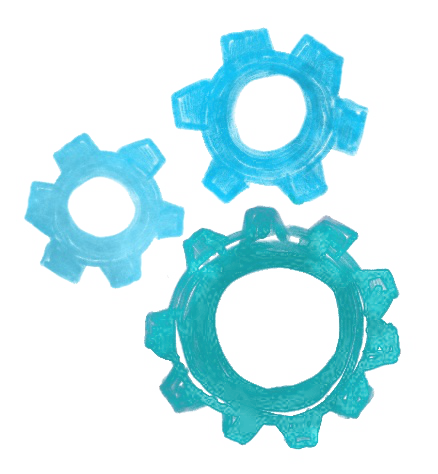
\includegraphics[height=.6cm]{images/gears.png}} \large \textcolor{deffun-text}{Definition-Box: #1}\\
    }
    {
  \end{mybox}
  }

% design
\newenvironment{design}[1][Title]
  {
  \setlength{\fboxsep}{1em}
  \begin{mybox}[design-line]
    \raisebox{-.2\height}{
\includegraphics[height=.6cm]{images/design.png}} \large \textcolor{design-text}{Approfondimento: #1}\\
    }
    {
  \end{mybox}
  }

% trick
\newenvironment{trick}[1][Title]
  {
  \setlength{\fboxsep}{1em}
  \begin{mybox}[trick-line]
    \raisebox{-.2\height}{
\includegraphics[height=.6cm]{images/hat.png}} \large \textcolor{trick-text}{Trick-Box: #1}\\
    }
    {
  \end{mybox}
  }
\usepackage{titlepic}
\titlepic{
\includegraphics[width=\textwidth]{images/logo_psicostat.pdf}}
\usepackage[]{natbib}
\bibliographystyle{plainnat}

\title{{Introduzione a R}}
\usepackage{etoolbox}
\makeatletter
\providecommand{\subtitle}[1]{% add subtitle to \maketitle
  \apptocmd{\@title}{\par {\large #1 \par}}{}{}
}
\makeatother
\subtitle{Corso per imparare le basi di \textbf{R}}
\author{\href{https://psicostat.dpss.psy.unipd.it/}{Psicostat}}
\date{11-03-2021}

\begin{document}
\maketitle

{
\setcounter{tocdepth}{1}
\tableofcontents
}
\hypertarget{presentazione}{%
\chapter*{Presentazione}\label{presentazione}}
\addcontentsline{toc}{chapter}{Presentazione}

In questo libro impareremo le basi di \emph{R}, uno dei migliori software per la visualizzazione e l'analisi statistica dei dati. Partiremo da zero intorducendo gli aspetti fondamentili di R e i concetti alla base di ogni linguaggio di programmazione che ti pemetteranno in seguito di approfondire e sviluppare le tue abilità in questo bellissimo mondo.

\hypertarget{perchuxe8-r}{%
\section*{Perchè R}\label{perchuxe8-r}}
\addcontentsline{toc}{section}{Perchè R}

Ci sono molte ragioni per cui scegliere R rispetto ad altri programmi usati per condurre le analisi statistiche. Innanzitutto è un linguaggio di programmazione (come ad esempio Python, Java, C++, o Julia) e non semplicemente un'interfaccia punta e clicca (come ad esempio SPSS o JASP). Questo comporta si maggiori difficoltà iniziali ma ti ricompenserà in futuro poichè avari imparato ad utilizza uno strumennto molto potente.

Inoltre, R è:

\begin{itemize}
\tightlist
\item
  nato per la statistica
\item
  open-source
\item
  ricco di pacchetti
\item
  supportato da una grande comunità
\item
  gratis
\end{itemize}

\hypertarget{struttura-del-libro}{%
\section*{Struttura del libro}\label{struttura-del-libro}}
\addcontentsline{toc}{section}{Struttura del libro}

Il libro è suddiviso in quattro sezioni principali:

\begin{itemize}
\tightlist
\item
  \textbf{Get started}. Una volta installato R ed RStudio, famiglierizzeremo con l'ambiente di lavoro introducendo alcuni aspetti generali e le funzioni principali. Verranno inoltre descritte alcune buone regole per iniziare una sessione di lavoro in R.
\item
  \textbf{Struttura dei dati}. Impareremo gli oggetti principali che R utilizza al suo interno. Variabili, vettori, matrici, dataframe e liste non avranno più segreti e capiremo come manipolarli e utlizzarli a seconda delle varie necessità.
\item
  \textbf{Algoritmi}. Non farti spaventare da questo nome. Ne avrai spesso sentito parlarne come qualcosa di molto complicato, ma in realtà gli algoritmi sono semplicemente una serie di istruzioni che il computer segue quando deve eseguire un determinato compito. In questa sezione vedremo i principali comandi di R usati per definire degli algoritmi. Questo è il vantaggio di conoscere un linguaggio di programmazione, ci permette di creare nuovi programmi che il computer eseguirà per noi.
\item
  \textbf{Case study}. Eseguiremo passo per passo un analisi che ci permetterà di imparare come importare i dati, codificare le variabili, manipolare e preprare i dati perle analisi, condurre delle analisi descrittive e creare dei grafici.
\end{itemize}

Alla fine di questo libro probabilmente non sarete assunti da Google, ma speriamo almeno che R non vi faccia più così paura e che magari a qualcuno sia nato l'interesse di approfondire questo fantastico mondo fatto di linee di codice.

\hypertarget{risorse-utili}{%
\section*{Risorse Utili}\label{risorse-utili}}
\addcontentsline{toc}{section}{Risorse Utili}

Segnaliamo qui per il lettore interessato del materiale online (in inglese) per approfondire le conoscenze sull'uso di R.

Materiale introduttivo:

\begin{itemize}
\tightlist
\item
  \emph{R for Psychological Science} di Danielle Navarro \url{https://psyr.djnavarro.net/index.html}
\item
  \emph{Hands-On Programming with R} di Garrett Grolemund \url{https://rstudio-education.github.io/hopr/}
\end{itemize}

Materiale intermedio:

\begin{itemize}
\tightlist
\item
  \emph{R for Data Science} di Hadley Wickham e Garrett Grolemund \url{https://r4ds.had.co.nz/}
\end{itemize}

Materiale avanzato:

\begin{itemize}
\tightlist
\item
  \emph{R Packages} di Hadley Wickham e Jennifer Bryan \url{https://r-pkgs.org/}
\item
  \emph{Advanced R} di Hadley Wickham \url{https://adv-r.hadley.nz/}
\end{itemize}

\hypertarget{psicostat}{%
\section*{Psicostat}\label{psicostat}}
\addcontentsline{toc}{section}{Psicostat}

Questo libro è stato prodotto da \textbf{Psicostat}, un gruppo di ricerca interdisciplinare dell'universita di Padova che unisce la passione per la statistica e la psicologia. Se vuoi conoscere di più riguardo le nostre attività visita il nosto sito \url{https://psicostat.dpss.psy.unipd.it/} o aggiungiti alla nostra mailing list \url{https://lists.dpss.psy.unipd.it/postorius/lists/psicostat.lists.dpss.psy.unipd.it/}.

\hypertarget{collaborazione}{%
\section*{Collaborazione}\label{collaborazione}}
\addcontentsline{toc}{section}{Collaborazione}

Se vuoi collaborare alla revione e scrittura di questo libro (ovviamente è tutto in R) visita la nostra repository di Github \url{https://github.com/psicostat/Introduction2R}.

\hypertarget{riconoscimenti}{%
\section*{Riconoscimenti}\label{riconoscimenti}}
\addcontentsline{toc}{section}{Riconoscimenti}

Il template di questo libro è basato su \href{https://github.com/rstudio/bookdown-demo}{Rstudio Bookdown-demo} rilasciato con licenza \href{https://creativecommons.org/publicdomain/zero/1.0/}{CC0-1.0} e \href{https://rstudio4edu.github.io/rstudio4edu-book/}{rstudio4edu-book} rilasciato con licenza \href{https://creativecommons.org/licenses/by/2.0/}{CC BY}. Nota che le illustrazioni utilizzate nelle vignette appartengono sempre a \href{https://rstudio4edu.github.io/rstudio4edu-book/}{rstudio4edu-book} e sono rilasciate con licenza \href{https://creativecommons.org/licenses/by-nc/2.0/}{CC BY-NC}.

\hypertarget{licenza}{%
\section*{Licenza}\label{licenza}}
\addcontentsline{toc}{section}{Licenza}

Questo libro è rilasciato sotto la Creative Commons Attribution-ShareAlike 4.0 International Public License (\href{https://creativecommons.org/licenses/by-sa/4.0/legalcode}{CC BY-SA}).
Le illustrazioni utilizzate nelle vignette appartengono a \href{https://rstudio4edu.github.io/rstudio4edu-book/}{rstudio4edu-book} e sono rilasciate con licenza \href{https://creativecommons.org/licenses/by-nc/2.0/}{CC BY-NC}.

\hypertarget{part-get-started}{%
\part*{Get Started}\label{part-get-started}}
\addcontentsline{toc}{part}{Get Started}

\hypertarget{intorduzione}{%
\chapter*{Intorduzione}\label{intorduzione}}
\addcontentsline{toc}{chapter}{Intorduzione}

In questa sezione verranno presentate le istruzioni per installare R ed RStudio. In seguito, famiglierizzeremo con l'ambiente di lavoro introducendo alcuni aspetti generali e le funzioni principali. Verranno inoltre descritte alcune buone regole per iniziare una sessione di lavoro in R.

I capitoli sono così organizzati:

\begin{itemize}
\tightlist
\item
  \textbf{Capitolo \ref{install}: Installare R e RStudio}. Instruzioni passo a passo per installare R e RStudio
\item
  \textbf{Capitolo \ref{rstudio-gui}: Interfaccia RStudio}. Introduzione all'interfaccia utente di RStudio.
\item
  \textbf{Capitolo \ref{first-comands}: Primi Passi in R}. Operatori matematici, operatori logici, creazione di variabili e utilizzo di funzioni.
\item
  \textbf{Capitolo \ref{working-session}: Sessione di Lavoro}. Utilizzo degli script e introduzione dei concetti di environment, working directory e pacchetti di R.
\end{itemize}

\hypertarget{install}{%
\chapter{Installare R e RStudio}\label{install}}

R ed R-studio sono due software distinti. R è un linguaggio di programmazione usato in particolare in ambiti quali la statistica. R-studio invece è un'interfaccia \emph{user-friendly} che permette di utilizzare R.
R può essere utilizzato autonomamente tuttavia è consigliato l'utilizzo attraverso R-studio. Entrambi vanno installati separatamente e la procedura varia a seconda del proprio sistema operativo (Windows, MacOS o Linux). Riportiamo le istruzioni solo per Windows e MacOS Linux (Ubuntu). Ovviamente R è disponibile per tutte le principali distribuzioni di Linux. Le istruzioni riportate per Ubuntu (la distribuzione più diffusa) sono valide anche per le distribuzioni derivate.

\hypertarget{installare-r}{%
\section{Installare R}\label{installare-r}}

\begin{enumerate}
\def\labelenumi{\arabic{enumi}.}
\tightlist
\item
  Accedere al sito \url{https://www.r-project.org}
\item
  Selezionare la voce \textbf{CRAN} (Comprehensive R Archive Network) dal menù di sinistra sotto \textbf{Download}
\end{enumerate}

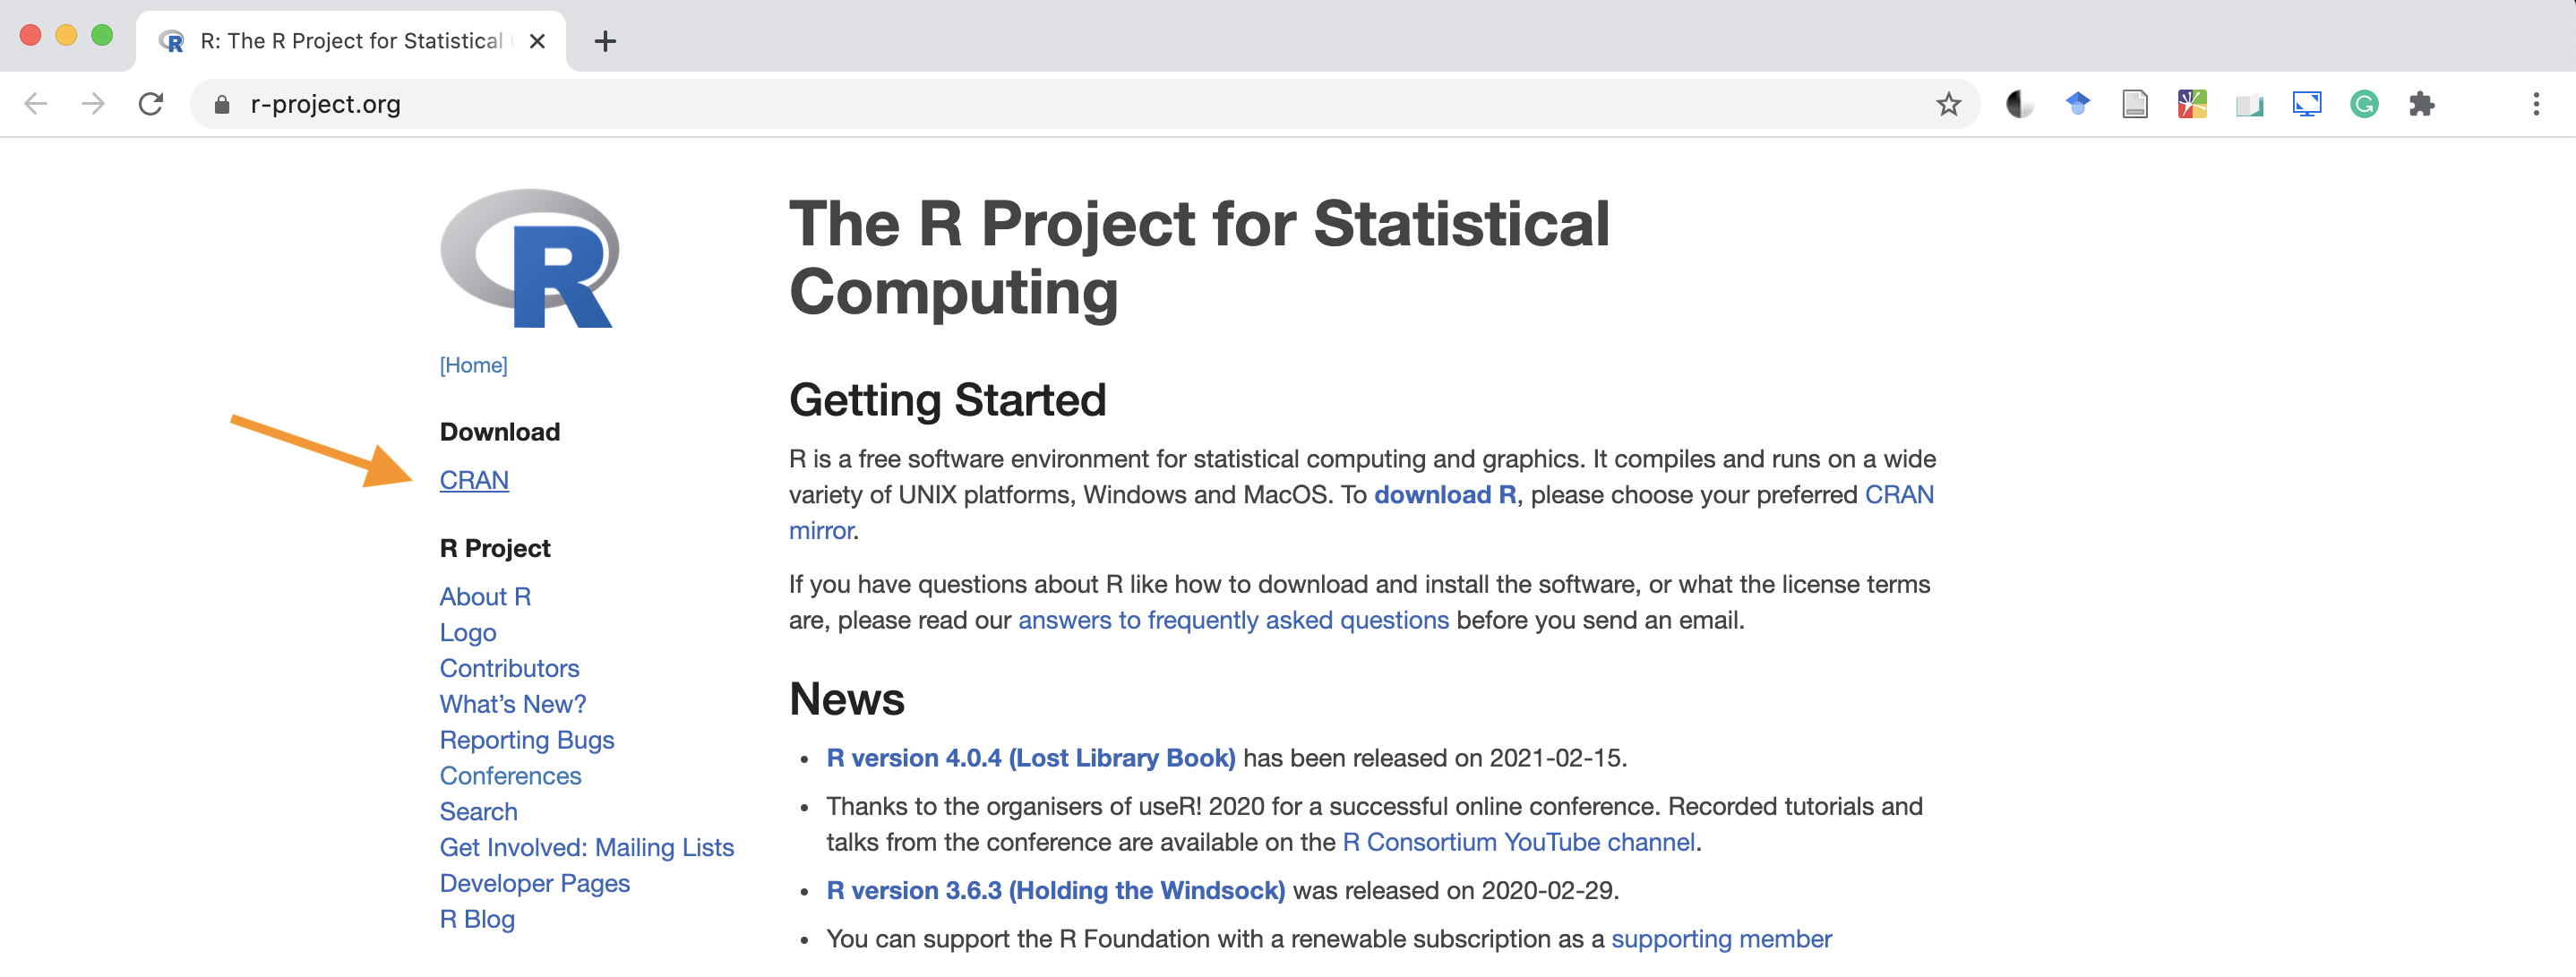
\includegraphics[width=0.95\textwidth,height=\textheight]{images/install_CRAN.png}

\begin{enumerate}
\def\labelenumi{\arabic{enumi}.}
\setcounter{enumi}{2}
\tightlist
\item
  Selezionare il primo link \url{https://cloud.r-project.org/}
\end{enumerate}

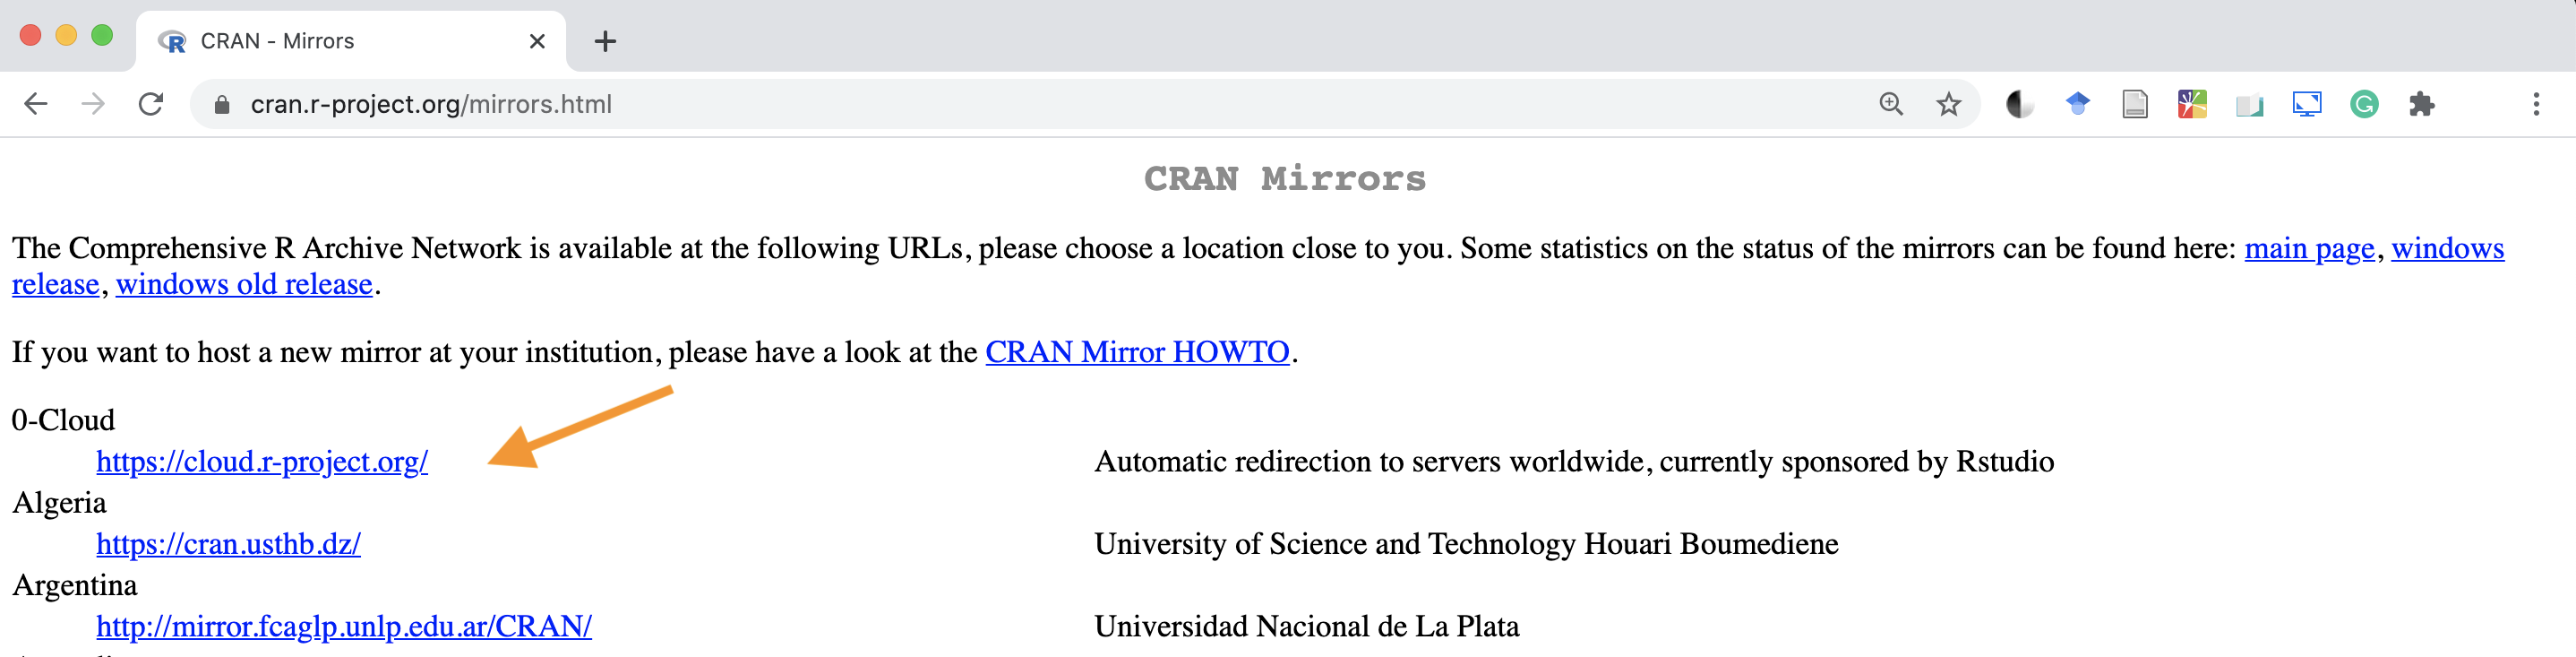
\includegraphics[width=0.95\textwidth,height=\textheight]{images/install_mirror.png}

\begin{enumerate}
\def\labelenumi{\arabic{enumi}.}
\setcounter{enumi}{3}
\tightlist
\item
  Selezionare il proprio sistema operativo
\end{enumerate}

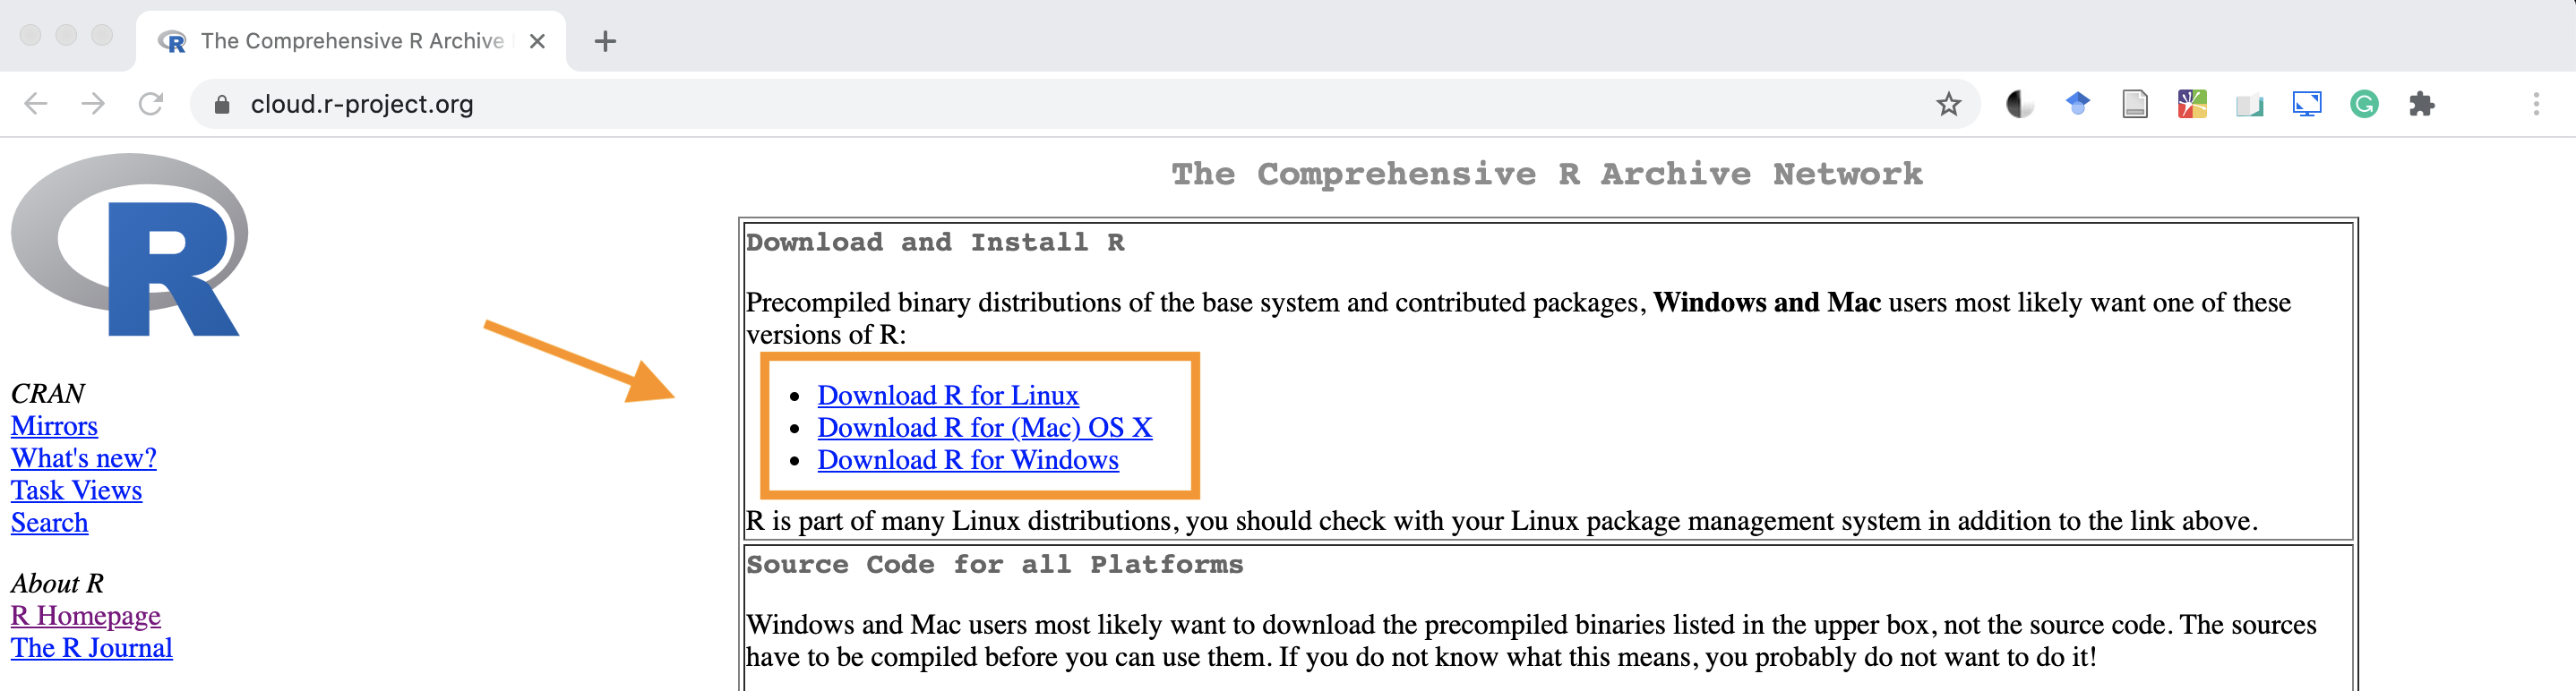
\includegraphics[width=0.95\textwidth,height=\textheight]{images/install_OS.png}

\hypertarget{r-windows}{%
\subsection{R Windows}\label{r-windows}}

\begin{enumerate}
\def\labelenumi{\arabic{enumi}.}
\tightlist
\item
  Selezionare la voce \textbf{base}
\end{enumerate}

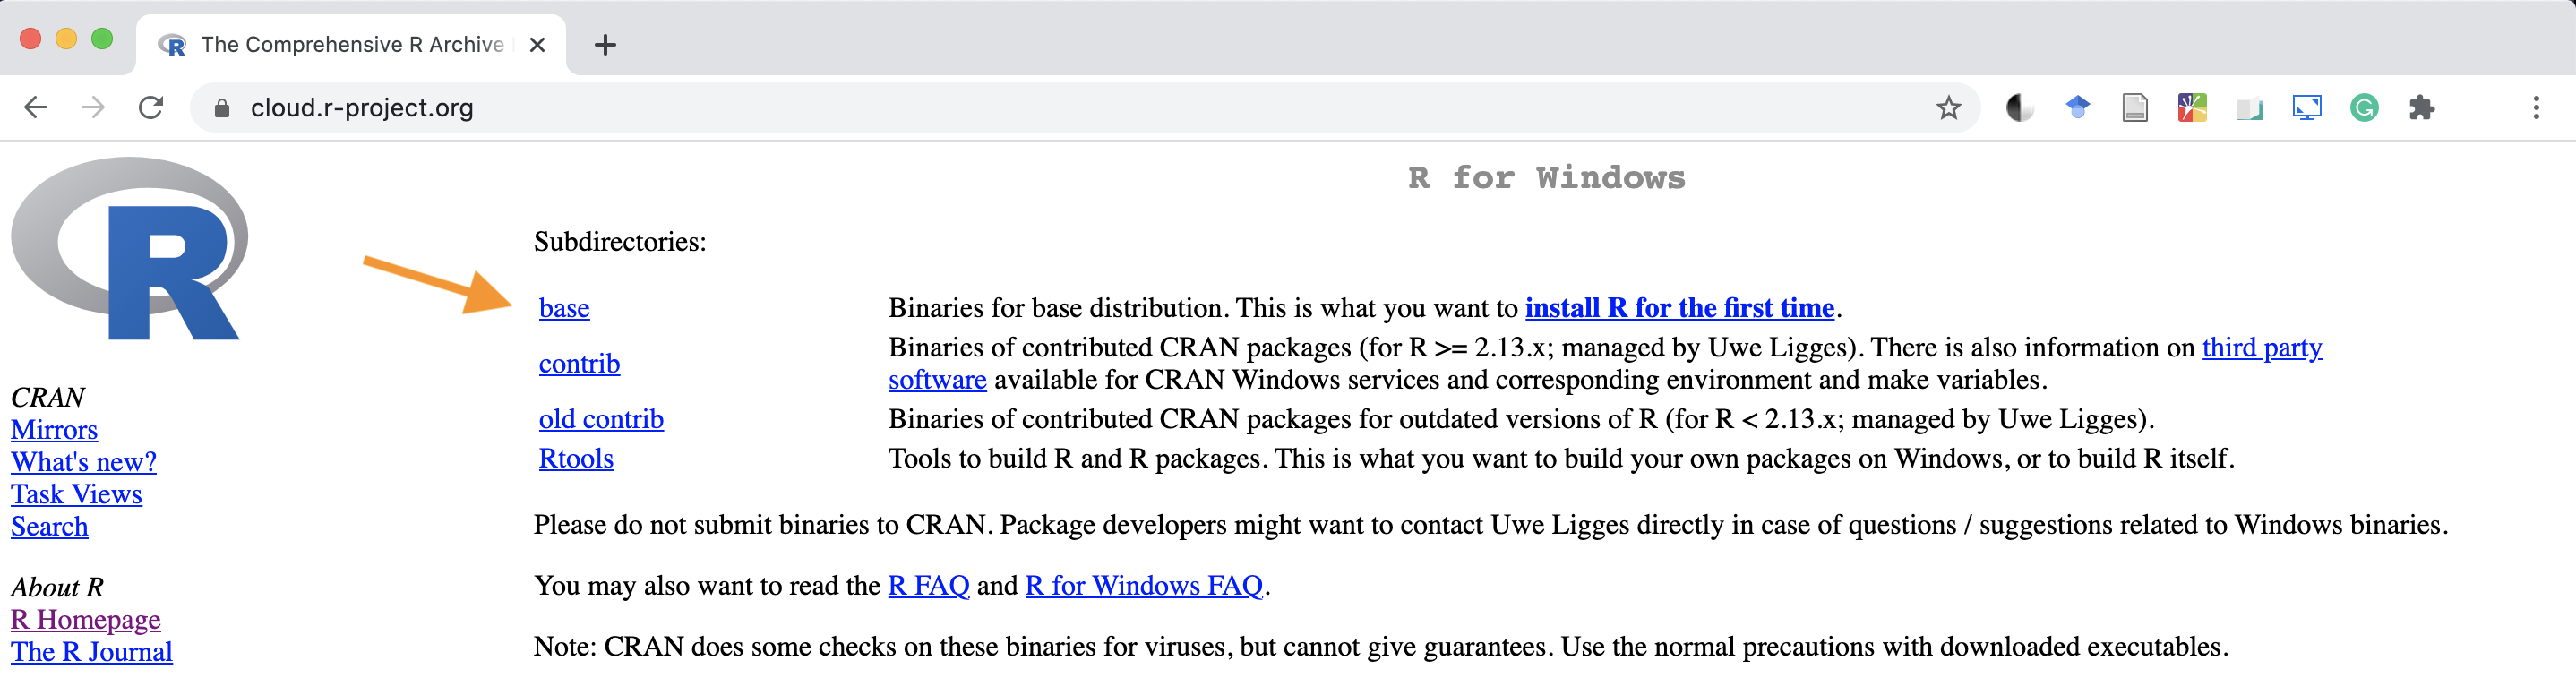
\includegraphics[width=0.95\textwidth,height=\textheight]{images/install-Windows-base.png}

\begin{enumerate}
\def\labelenumi{\arabic{enumi}.}
\setcounter{enumi}{1}
\tightlist
\item
  Selezionare la voce \textbf{Download} della versione più recente di R disponibile
\end{enumerate}

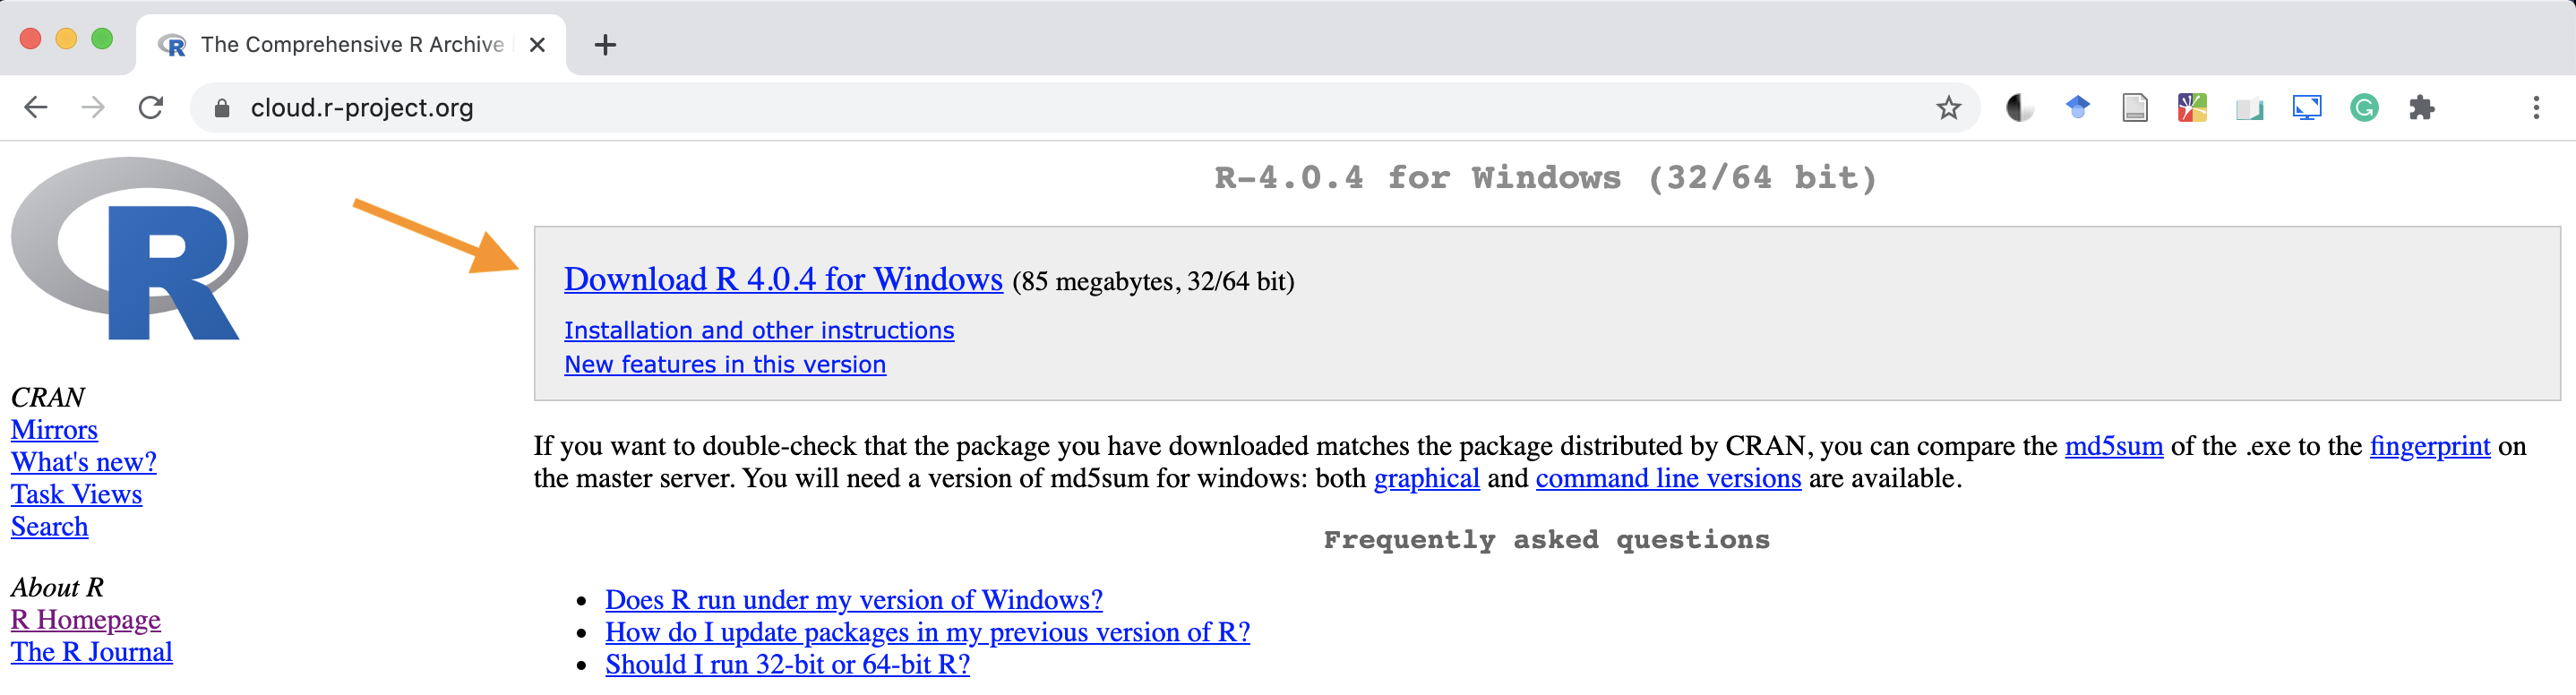
\includegraphics[width=0.95\textwidth,height=\textheight]{images/install-Windows-version.png}

\begin{enumerate}
\def\labelenumi{\arabic{enumi}.}
\setcounter{enumi}{2}
\tightlist
\item
  Al termine del download, eseguire il file e seguire le istruzioni fino al termine dell'installazione
\end{enumerate}

\hypertarget{r-macos}{%
\subsection{R MacOS}\label{r-macos}}

\begin{enumerate}
\def\labelenumi{\arabic{enumi}.}
\tightlist
\item
  Selezionare della versione più recente di R disponibile
\end{enumerate}

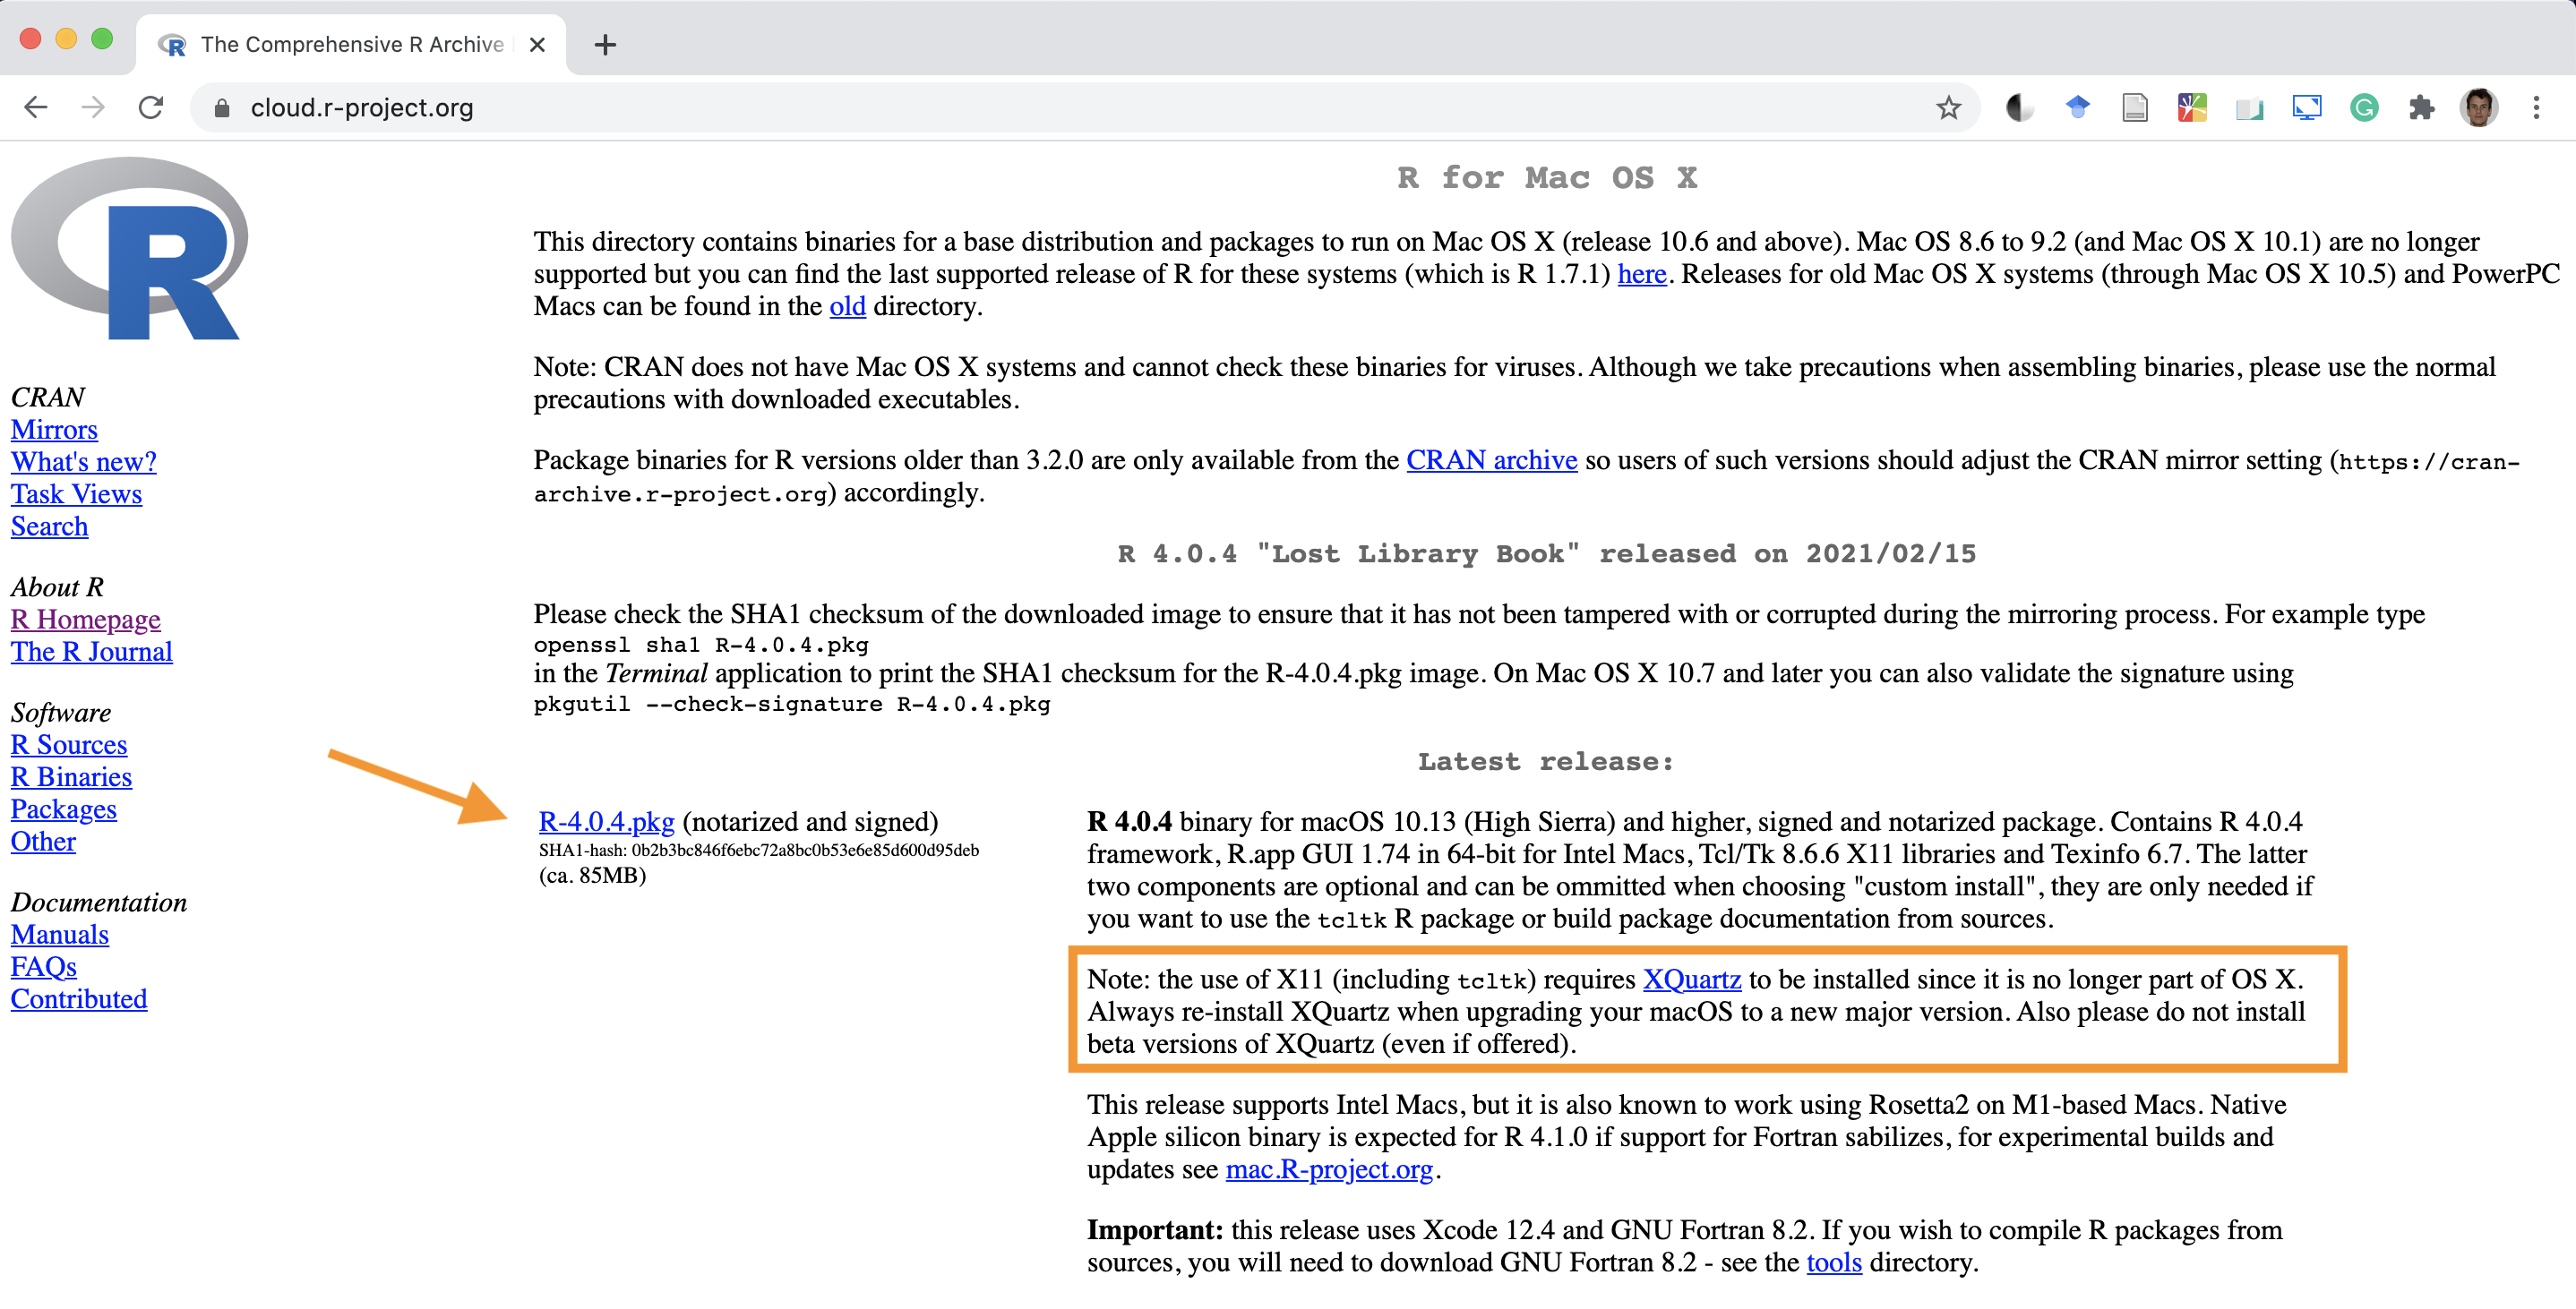
\includegraphics[width=0.95\textwidth,height=\textheight]{images/install_Mac_version.png}

\begin{enumerate}
\def\labelenumi{\arabic{enumi}.}
\setcounter{enumi}{1}
\tightlist
\item
  Al termine del download, eseguire il file e seguire le istruzioni fino al termine dell'installazione di R
\item
  Successivamente è necessario installare anche una componente aggiuntiva \textbf{XQuartz} premendo il link all'interno del riquadro arancione riportato nella figura precedente
\item
  Selezionare la voce Download
\end{enumerate}

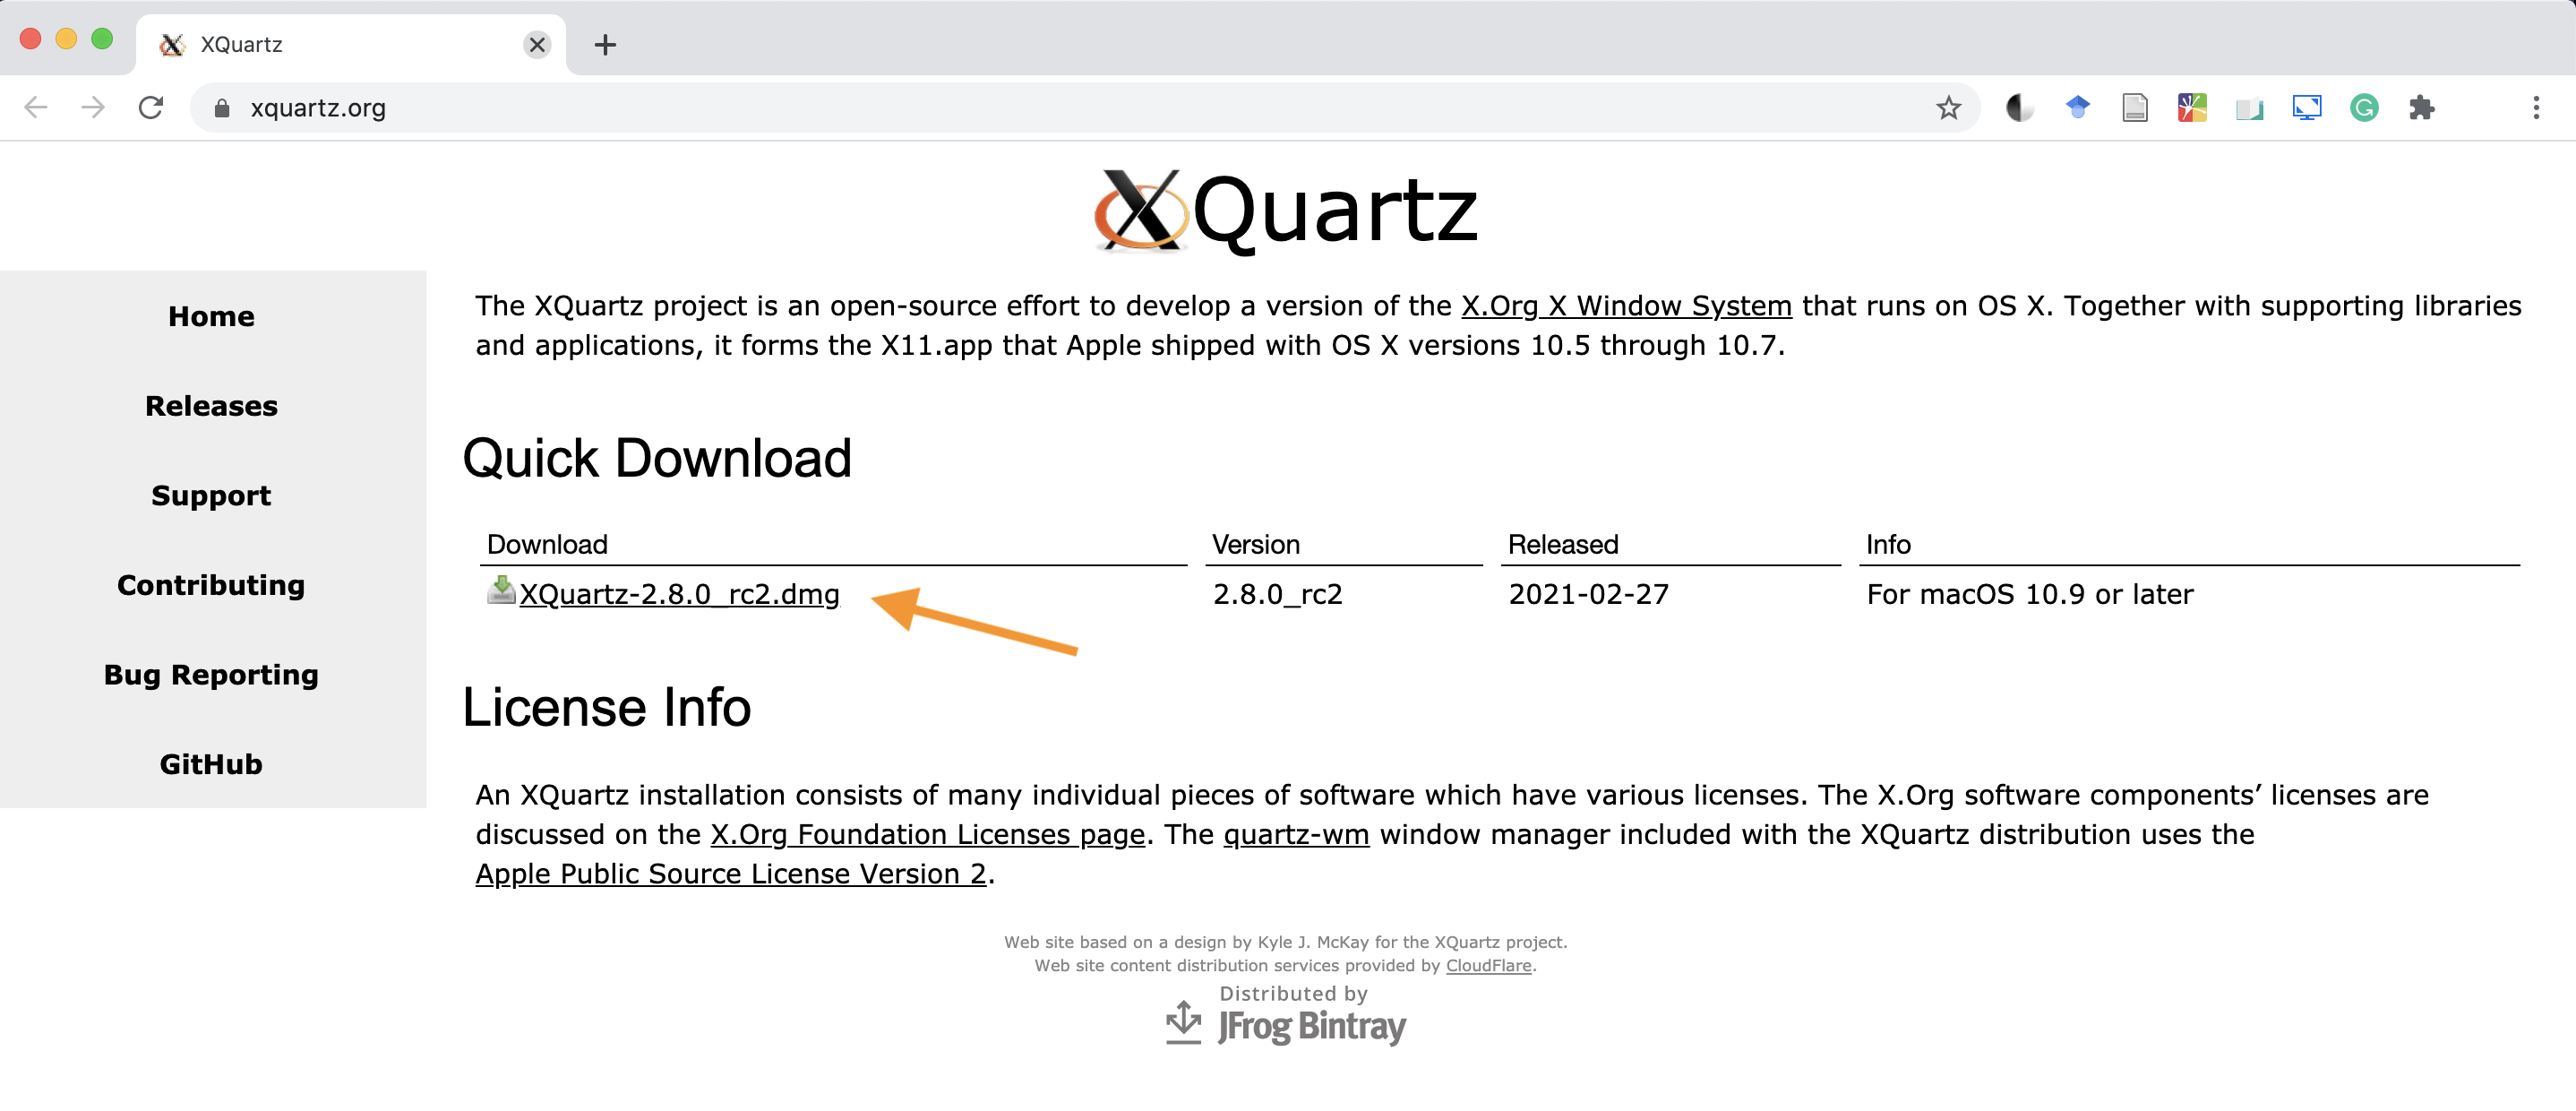
\includegraphics[width=0.95\textwidth,height=\textheight]{images/install_Mac_XQuartz.png}

\begin{enumerate}
\def\labelenumi{\arabic{enumi}.}
\setcounter{enumi}{4}
\tightlist
\item
  Al termine del download, eseguire il file e seguire le istruzioni fino al termine dell'installazione
\end{enumerate}

\hypertarget{r-linux}{%
\subsection{R Linux}\label{r-linux}}

Nonostante la semplicità di installazione di pacchetti su Linux, R a volte potrebbe essere più complicato da installare per via delle diverse distribuzioni, repository e chiavi per riconoscere la repository come sicura.

Sul \textbf{CRAN} vi è la guida ufficiale con tutti i comandi \texttt{apt} da eseguire da terminale. Seguendo questi passaggi non dovrebbero esserci problemi.

\begin{enumerate}
\def\labelenumi{\arabic{enumi}.}
\tightlist
\item
  Andate sul \href{https://cran.r-project.org/}{CRAN}
\item
  Cliccate \texttt{Download\ R\ for\ Linux}
\item
  Selezionate la vostra distribuzione (Ubuntu in questo caso)
\item
  Seguite le istruzioni, principalmente eseguendo i comandi da terminale suggeriti
\end{enumerate}

Per qualsiasi difficoltà o errore, sopratutto con il mondo Linux, una ricerca su online risolve sempre il problema.

\begin{design}[R Tools]

Utilizzi avanzati di R richiedono l'insallazione di una serie ulteriore software definiti \textbf{R tools}.

\hypertarget{windows}{%
\subsubsection*{Windows}\label{windows}}
\addcontentsline{toc}{subsubsection}{Windows}

Seleziona la voce \textbf{Rtools} e segui le istruzioni per completare l'installazione.

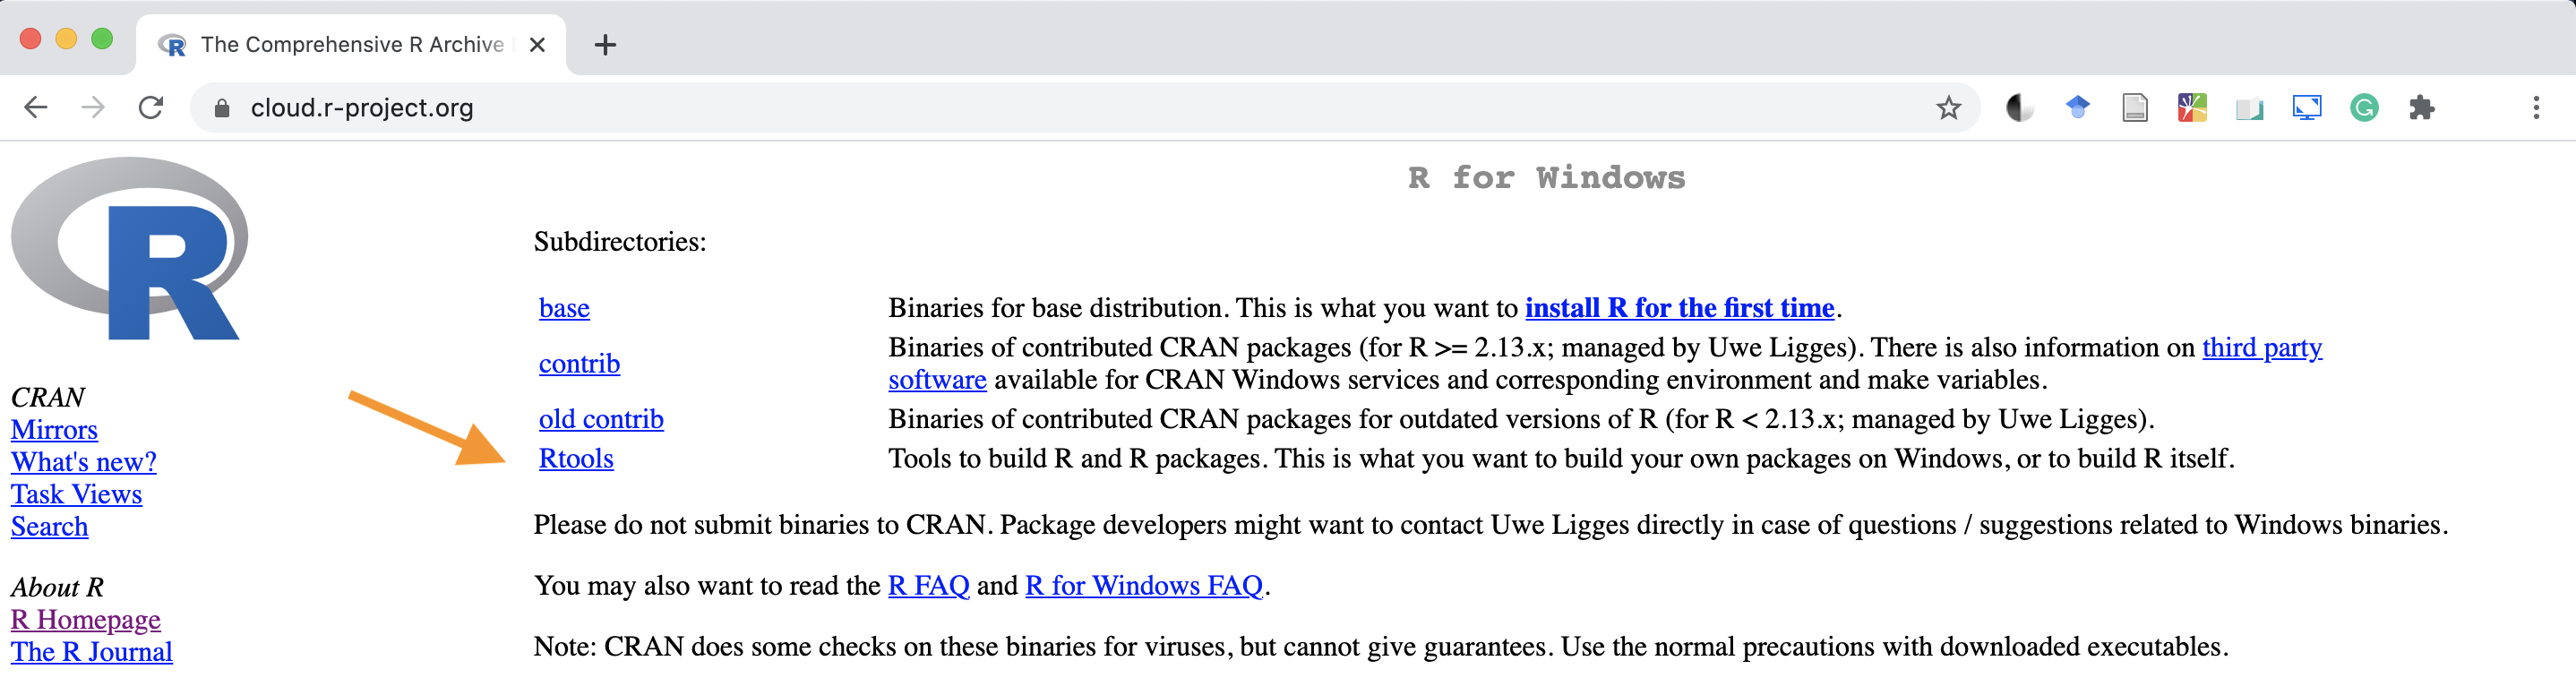
\includegraphics[width=0.95\textwidth,height=\textheight]{images/install-Windows-tools.png}

Nota che sono richieste anche delle operazioni di configurazione affinchè tutto funzioni correttamente.

\hypertarget{macos}{%
\subsubsection*{MacOS}\label{macos}}
\addcontentsline{toc}{subsubsection}{MacOS}

Seleziona la voce \textbf{tools} e segui le istruzioni riportate.

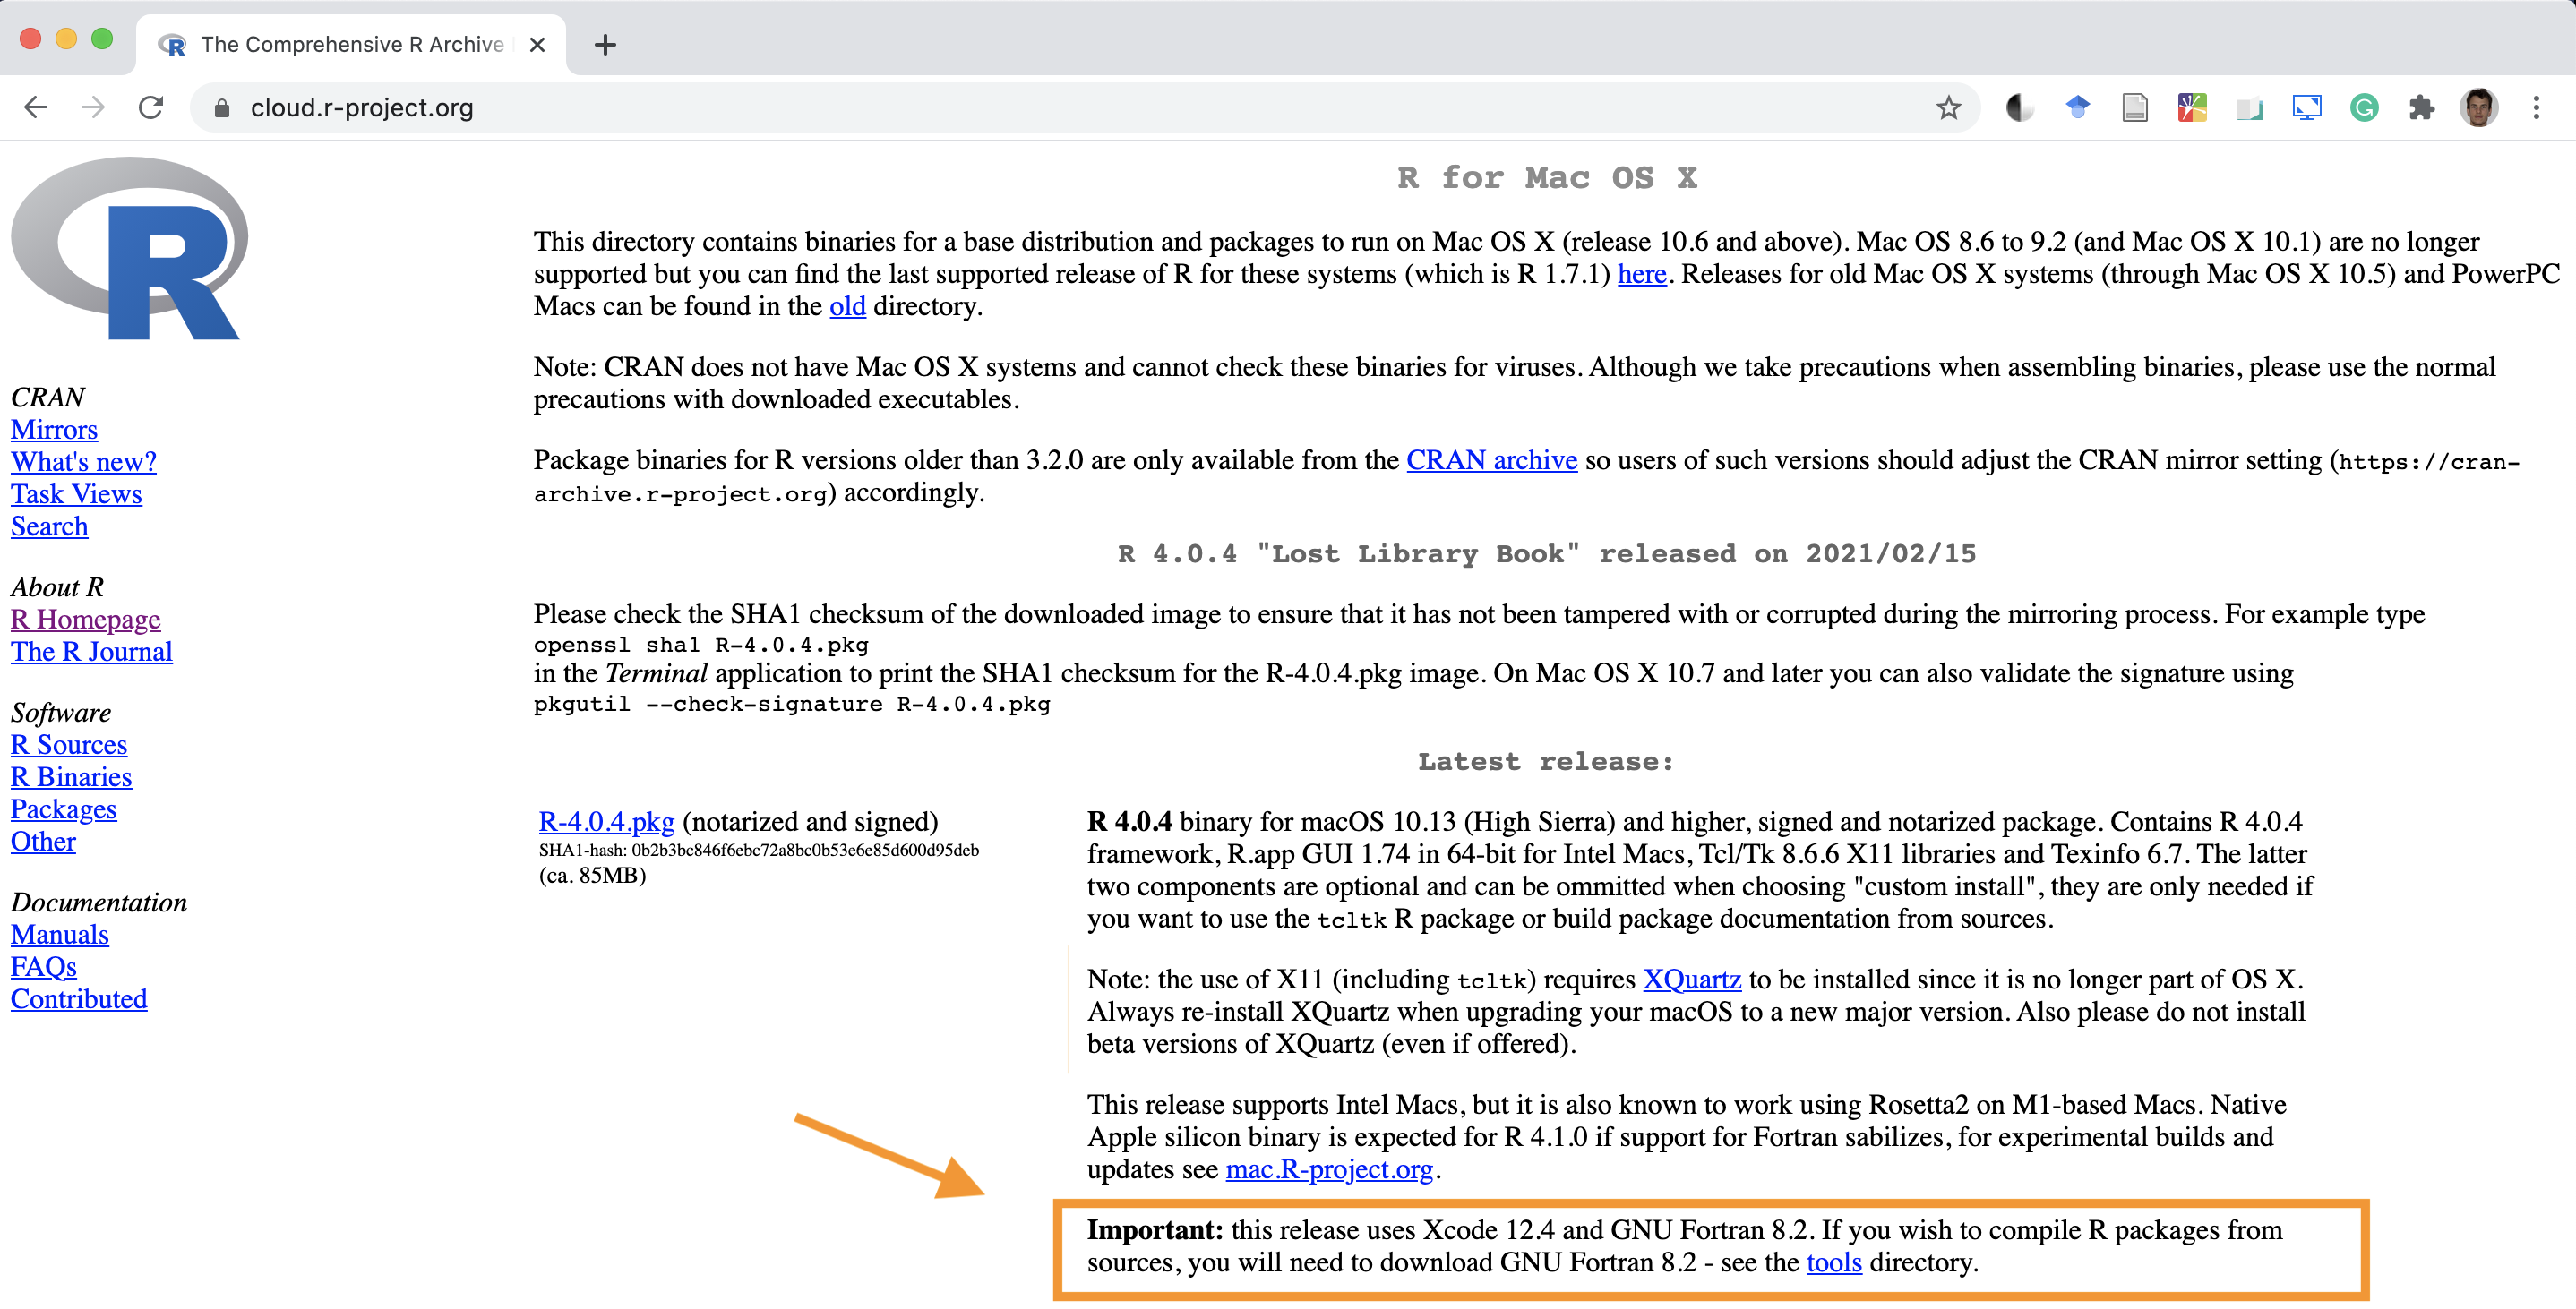
\includegraphics[width=0.95\textwidth,height=\textheight]{images/install_Mac_tools.png}

Nota in particolare che con R 4.0 le seguenti indicazioni sono riportate.

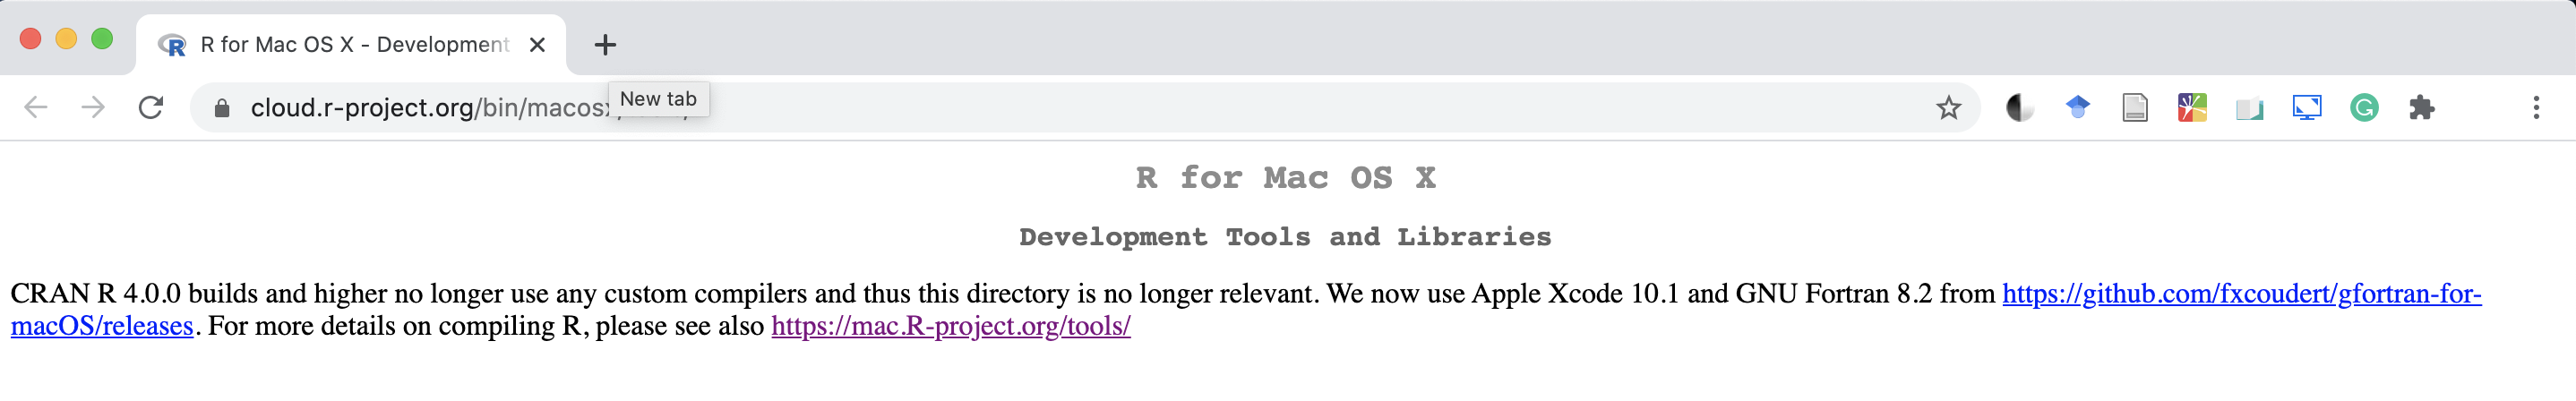
\includegraphics[width=0.95\textwidth,height=\textheight]{images/install_Mac_tools2.png}

\end{design}

\hypertarget{installare-r-studio}{%
\section{Installare R Studio}\label{installare-r-studio}}

\begin{enumerate}
\def\labelenumi{\arabic{enumi}.}
\tightlist
\item
  Accedere al sito \url{https://rstudio.com}
\item
  Selezionare la voce \textbf{DOWNLOAD IT NOW}
\end{enumerate}

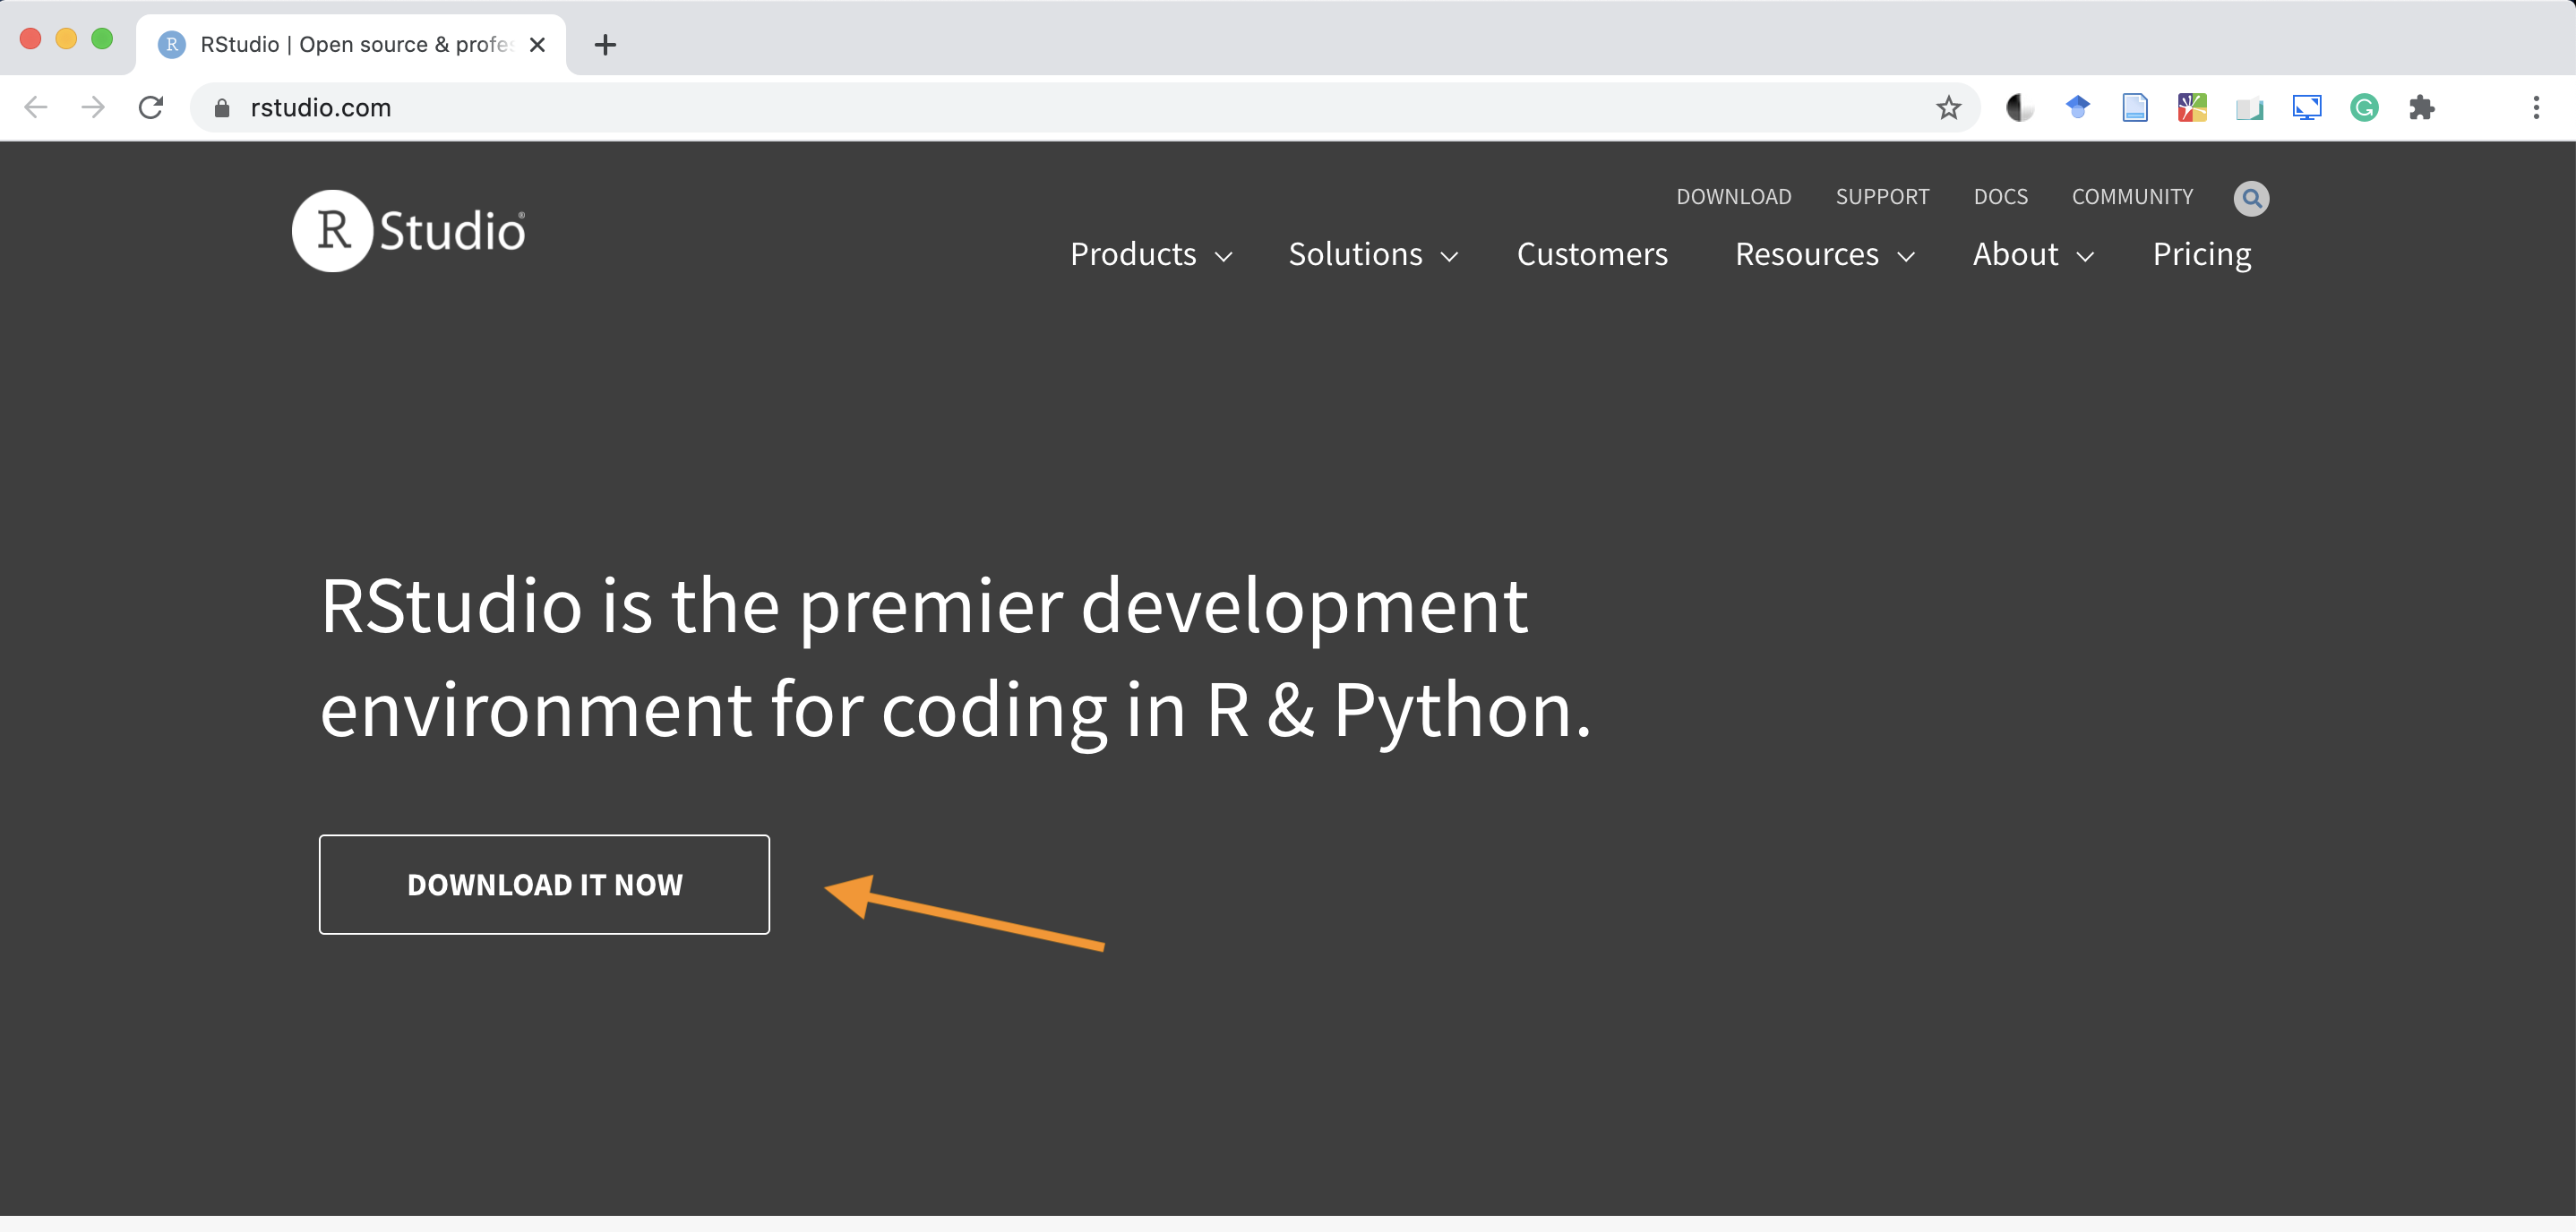
\includegraphics[width=0.95\textwidth,height=\textheight]{images/install_rstudio1.png}

\begin{enumerate}
\def\labelenumi{\arabic{enumi}.}
\setcounter{enumi}{2}
\tightlist
\item
  Selezionare la versione gratuita di RStudio Desktop
\end{enumerate}

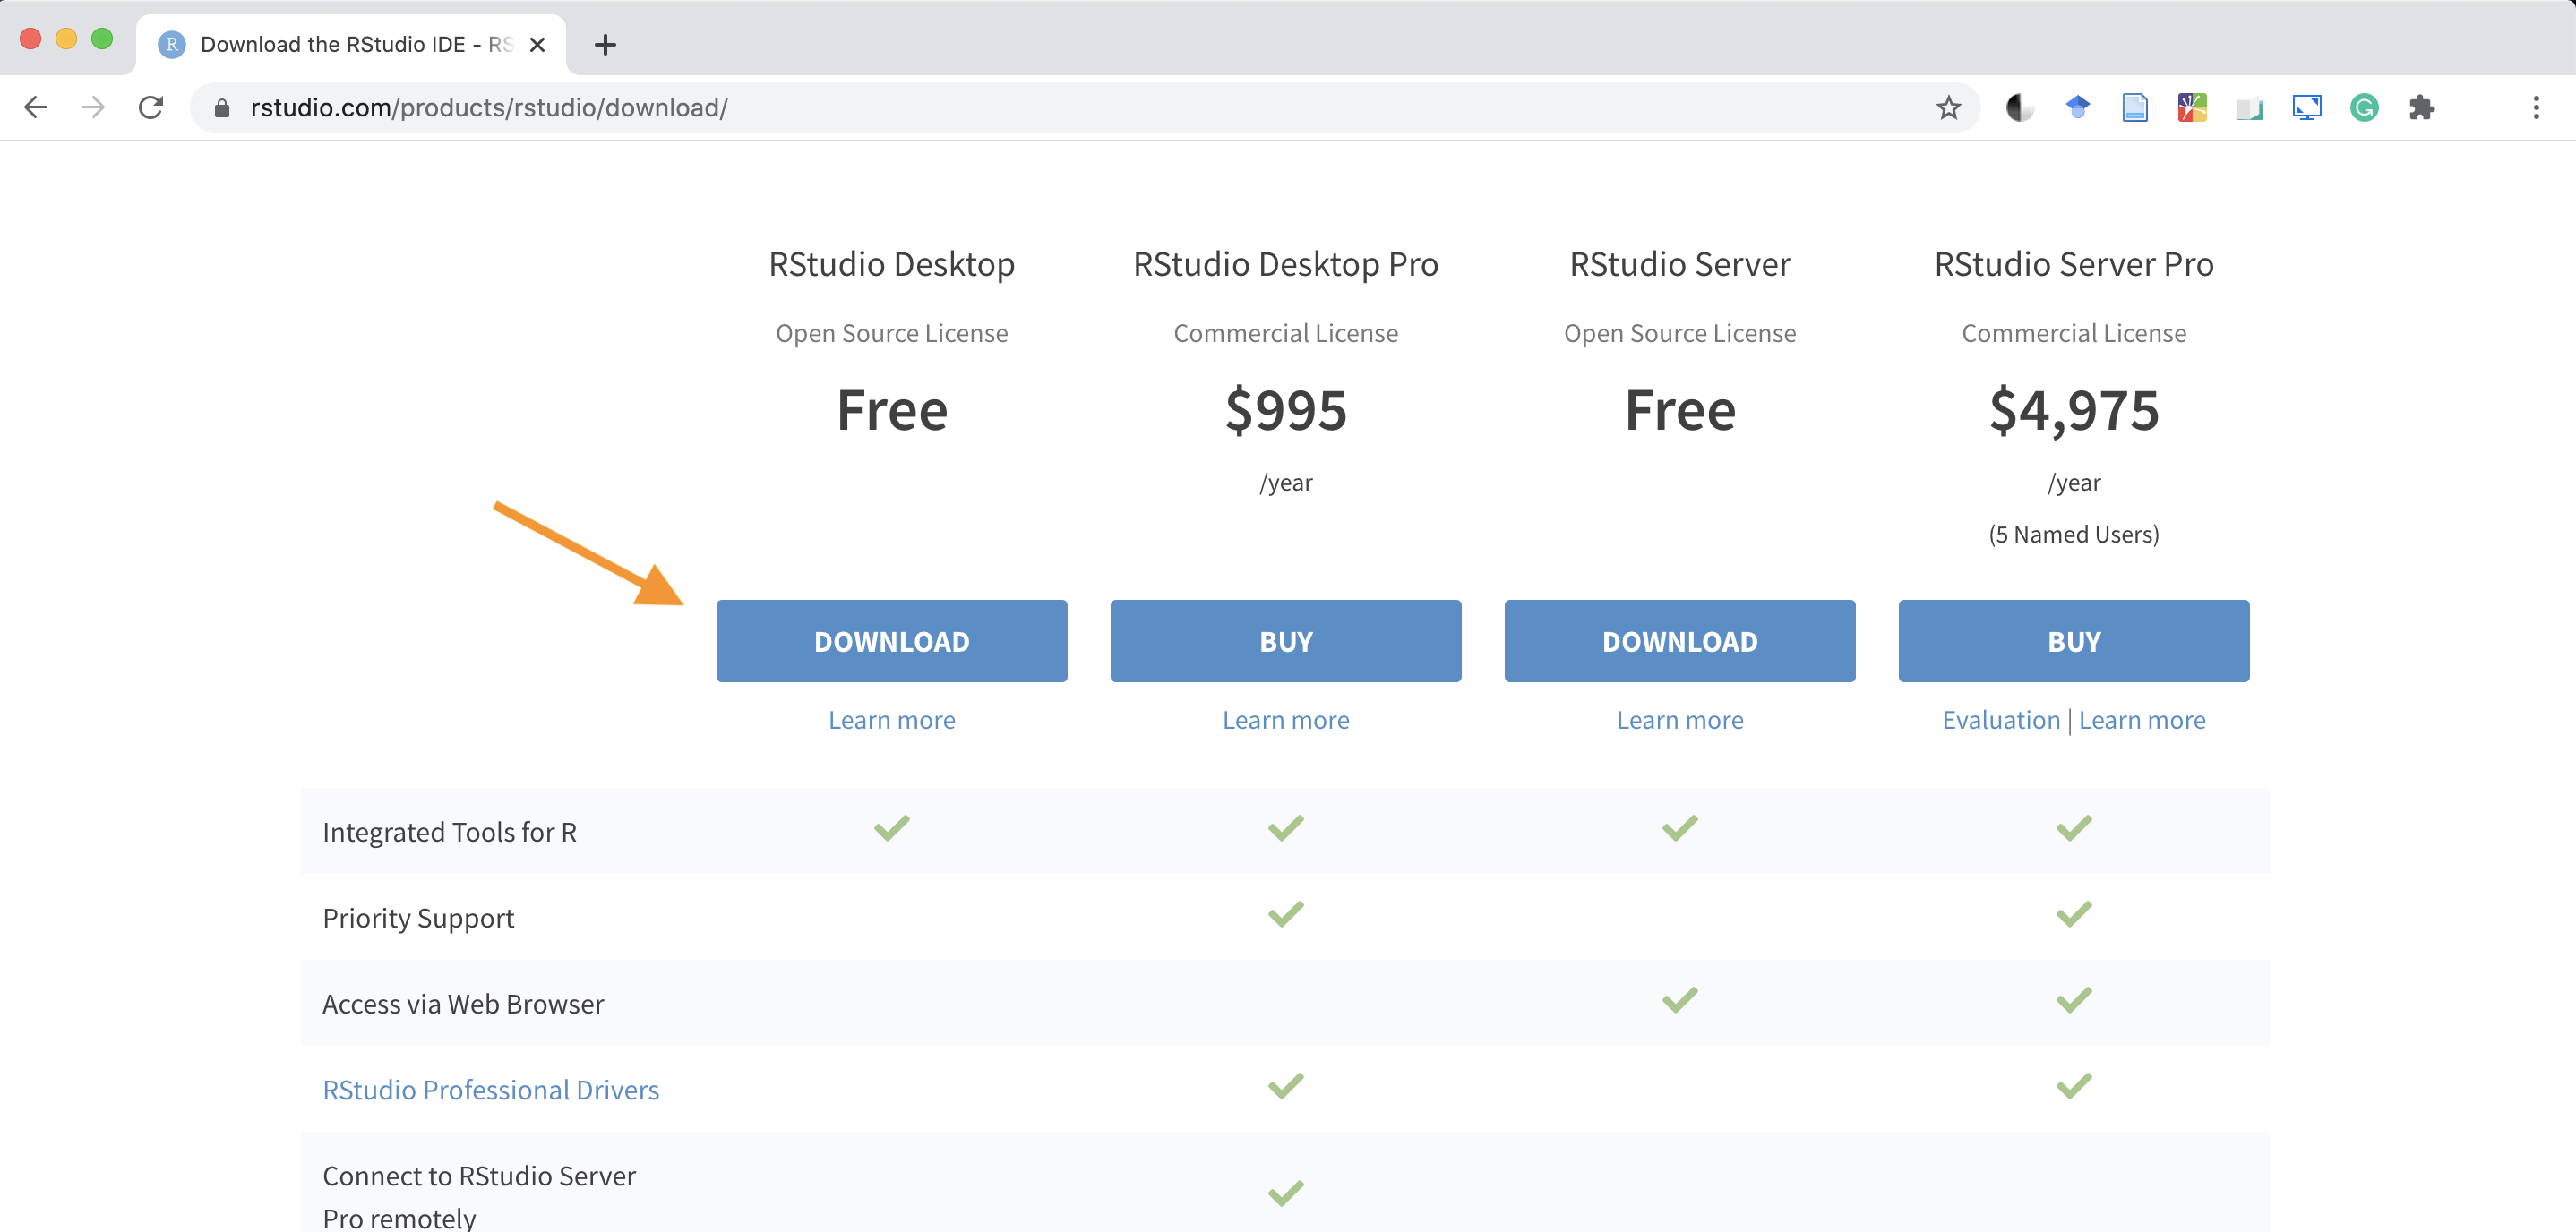
\includegraphics[width=0.95\textwidth,height=\textheight]{images/install_rstudio2.png}

\begin{enumerate}
\def\labelenumi{\arabic{enumi}.}
\setcounter{enumi}{3}
\tightlist
\item
  Selezionare la versione corretta a seconda del proprio sistema operativo
\end{enumerate}

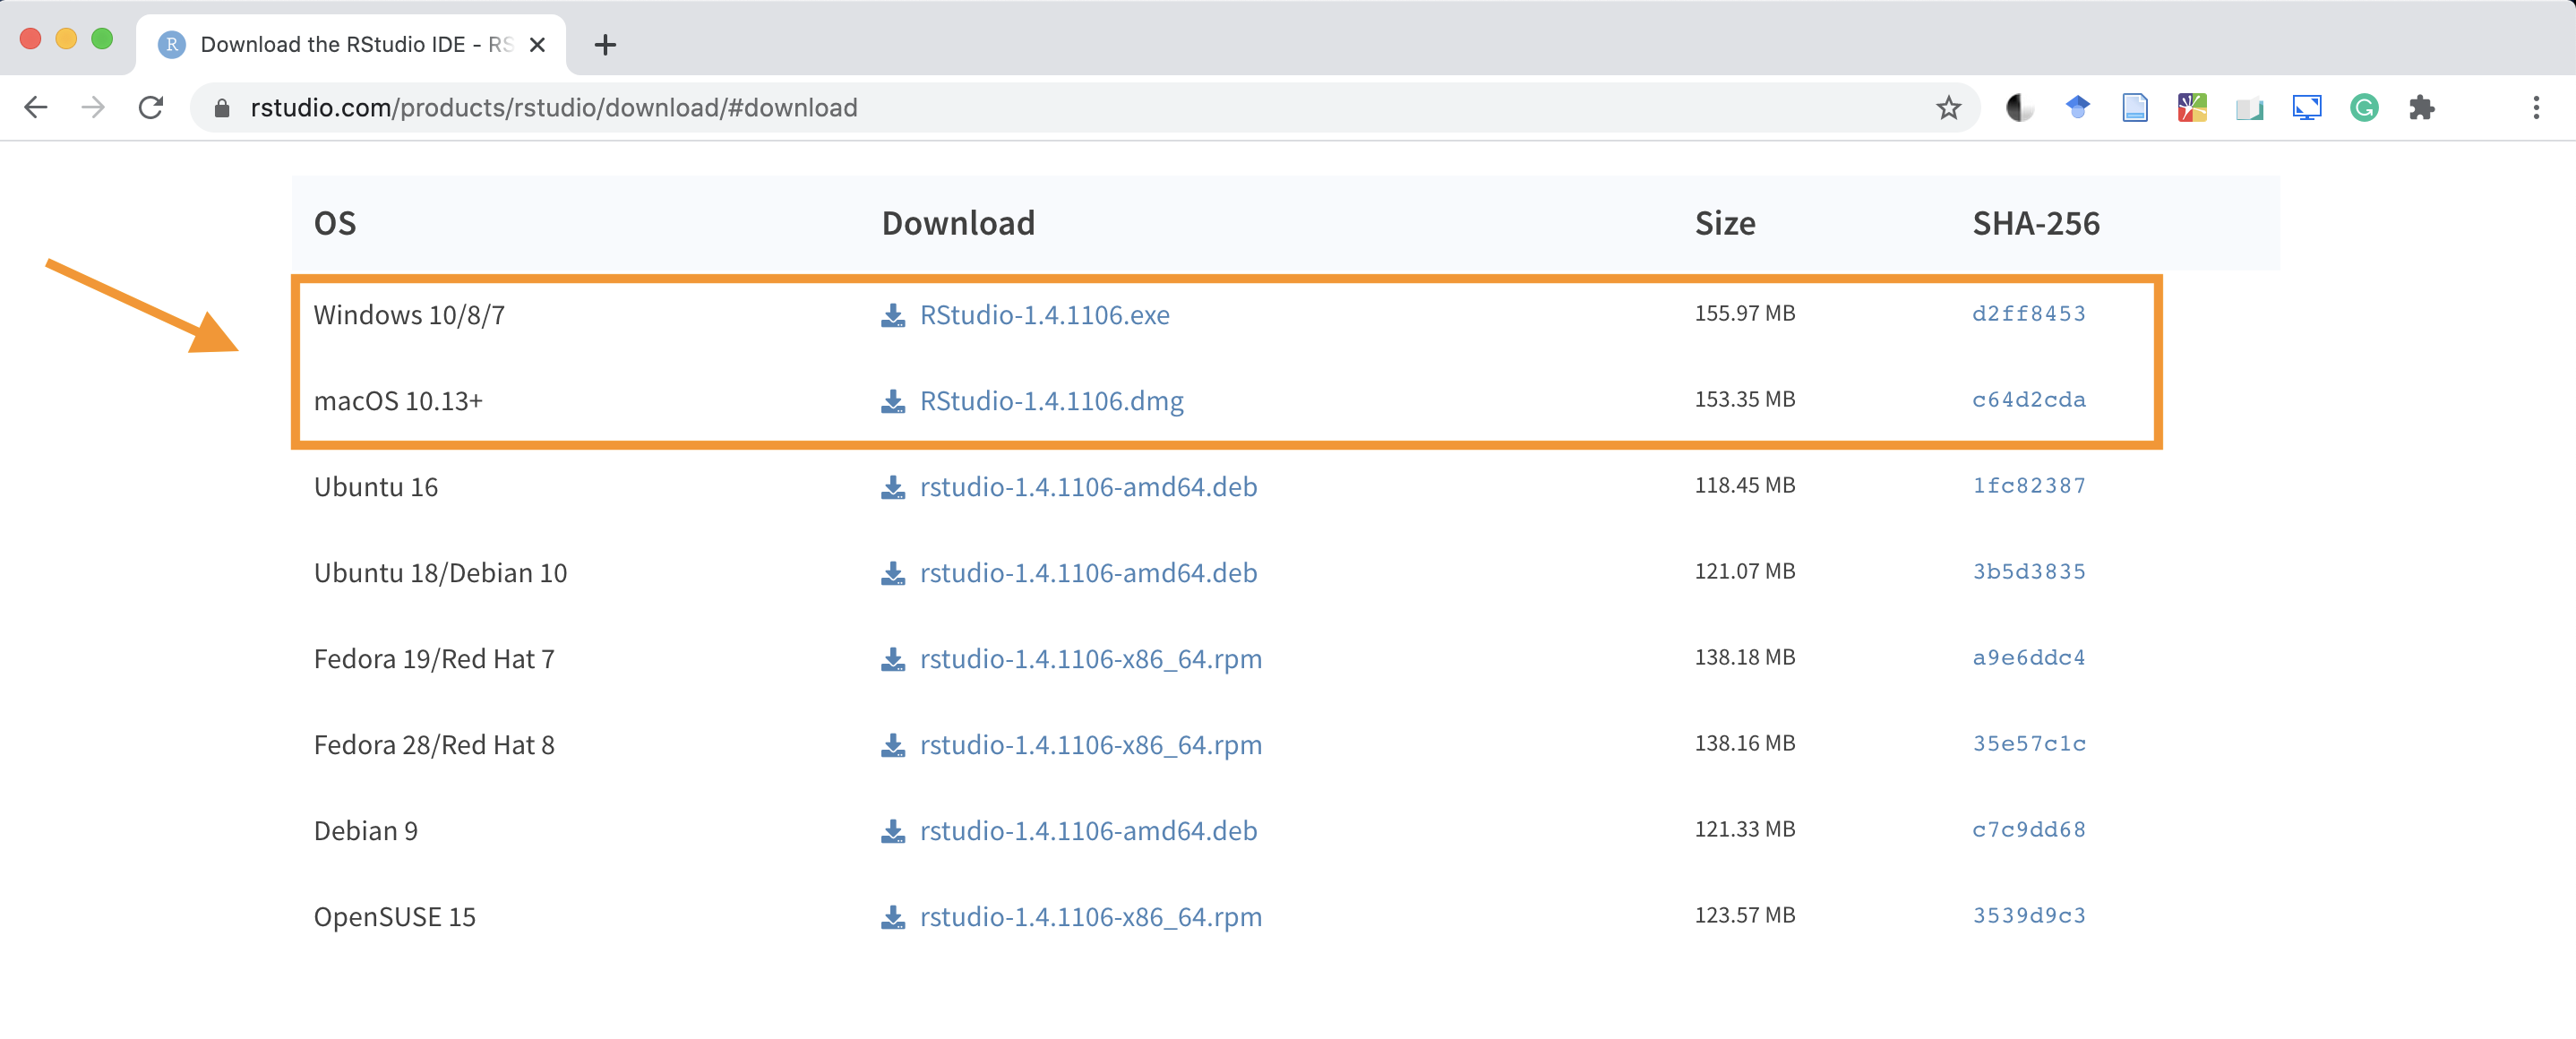
\includegraphics[width=0.95\textwidth,height=\textheight]{images/install_rstudio3.png}

\begin{enumerate}
\def\labelenumi{\arabic{enumi}.}
\setcounter{enumi}{4}
\tightlist
\item
  Al termine del download, eseguire il file e seguire le istruzioni fino al termine dell'installazione
\end{enumerate}

\hypertarget{r-studio-in-linux}{%
\subsection{R Studio in Linux}\label{r-studio-in-linux}}

In questo caso, come su Windows e MacOS l'installazione consiste nello scaricare ed eseguire il file corretto, in base alla distribuzione (ad esempio \texttt{.deb} per Ubuntu e derivate). Importante, nel caso di Ubuntu (ma dovrebbe valere anche per le altre distribuzioni) anche versioni successive a quella indicata (es. Ubuntu 16) sono perfettamente compatibili.

\hypertarget{rstudio-gui}{%
\chapter{Interfaccia RStudio}\label{rstudio-gui}}

In questo capitolo presenteremo l'interfaccia utente di RStudio. Molti aspetti che introdurremo brevemente qui verranno discussi nei sucessivi capitoli. Adesso ci interessa solo famigliarizzare con l'interfaccia del nostro strumento di lavoro principale ovvero RStudio.

Come abbiamo visto nel Capitolo \ref{install}, R è il vero ``motore computazionale'' che ci permette di compiere tutte le operazioni di calcolo, analisi statistiche e magie varie. Tuttavia l'interfaccia di base di R, definita \textbf{Console} (vedi Figura \ref{fig:r-console}), è per così dire \emph{démodé} o meglio, solo per veri intenditori.

\begin{figure}

{\centering 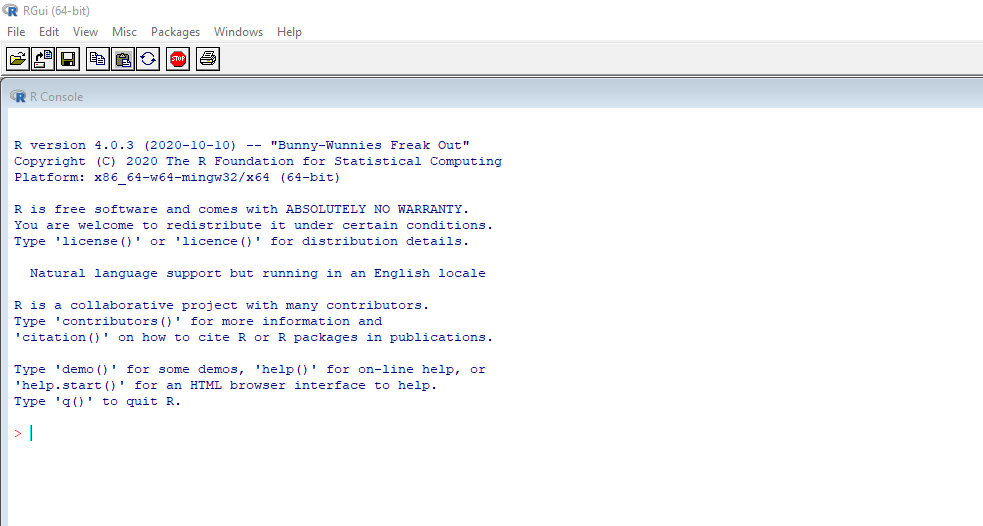
\includegraphics[width=0.85\linewidth]{images/r-console} 

}

\caption{La console di R, solo per veri intenditori}\label{fig:r-console}
\end{figure}

In genere, per lavorare con R viene utilizzato RStudio. RStudio è un programma (IDE - Integrated Development Environment) che integra in un unica interfaccia utente (GUI - Graphical User Interface) diversi strumenti utili per la scrittura ed esecuzione di codici. L'interfaccia di RStudio è costituita da 4 pannelli principali (vedi Figura \ref{fig:rstudio-gui}):

\begin{figure}

{\centering 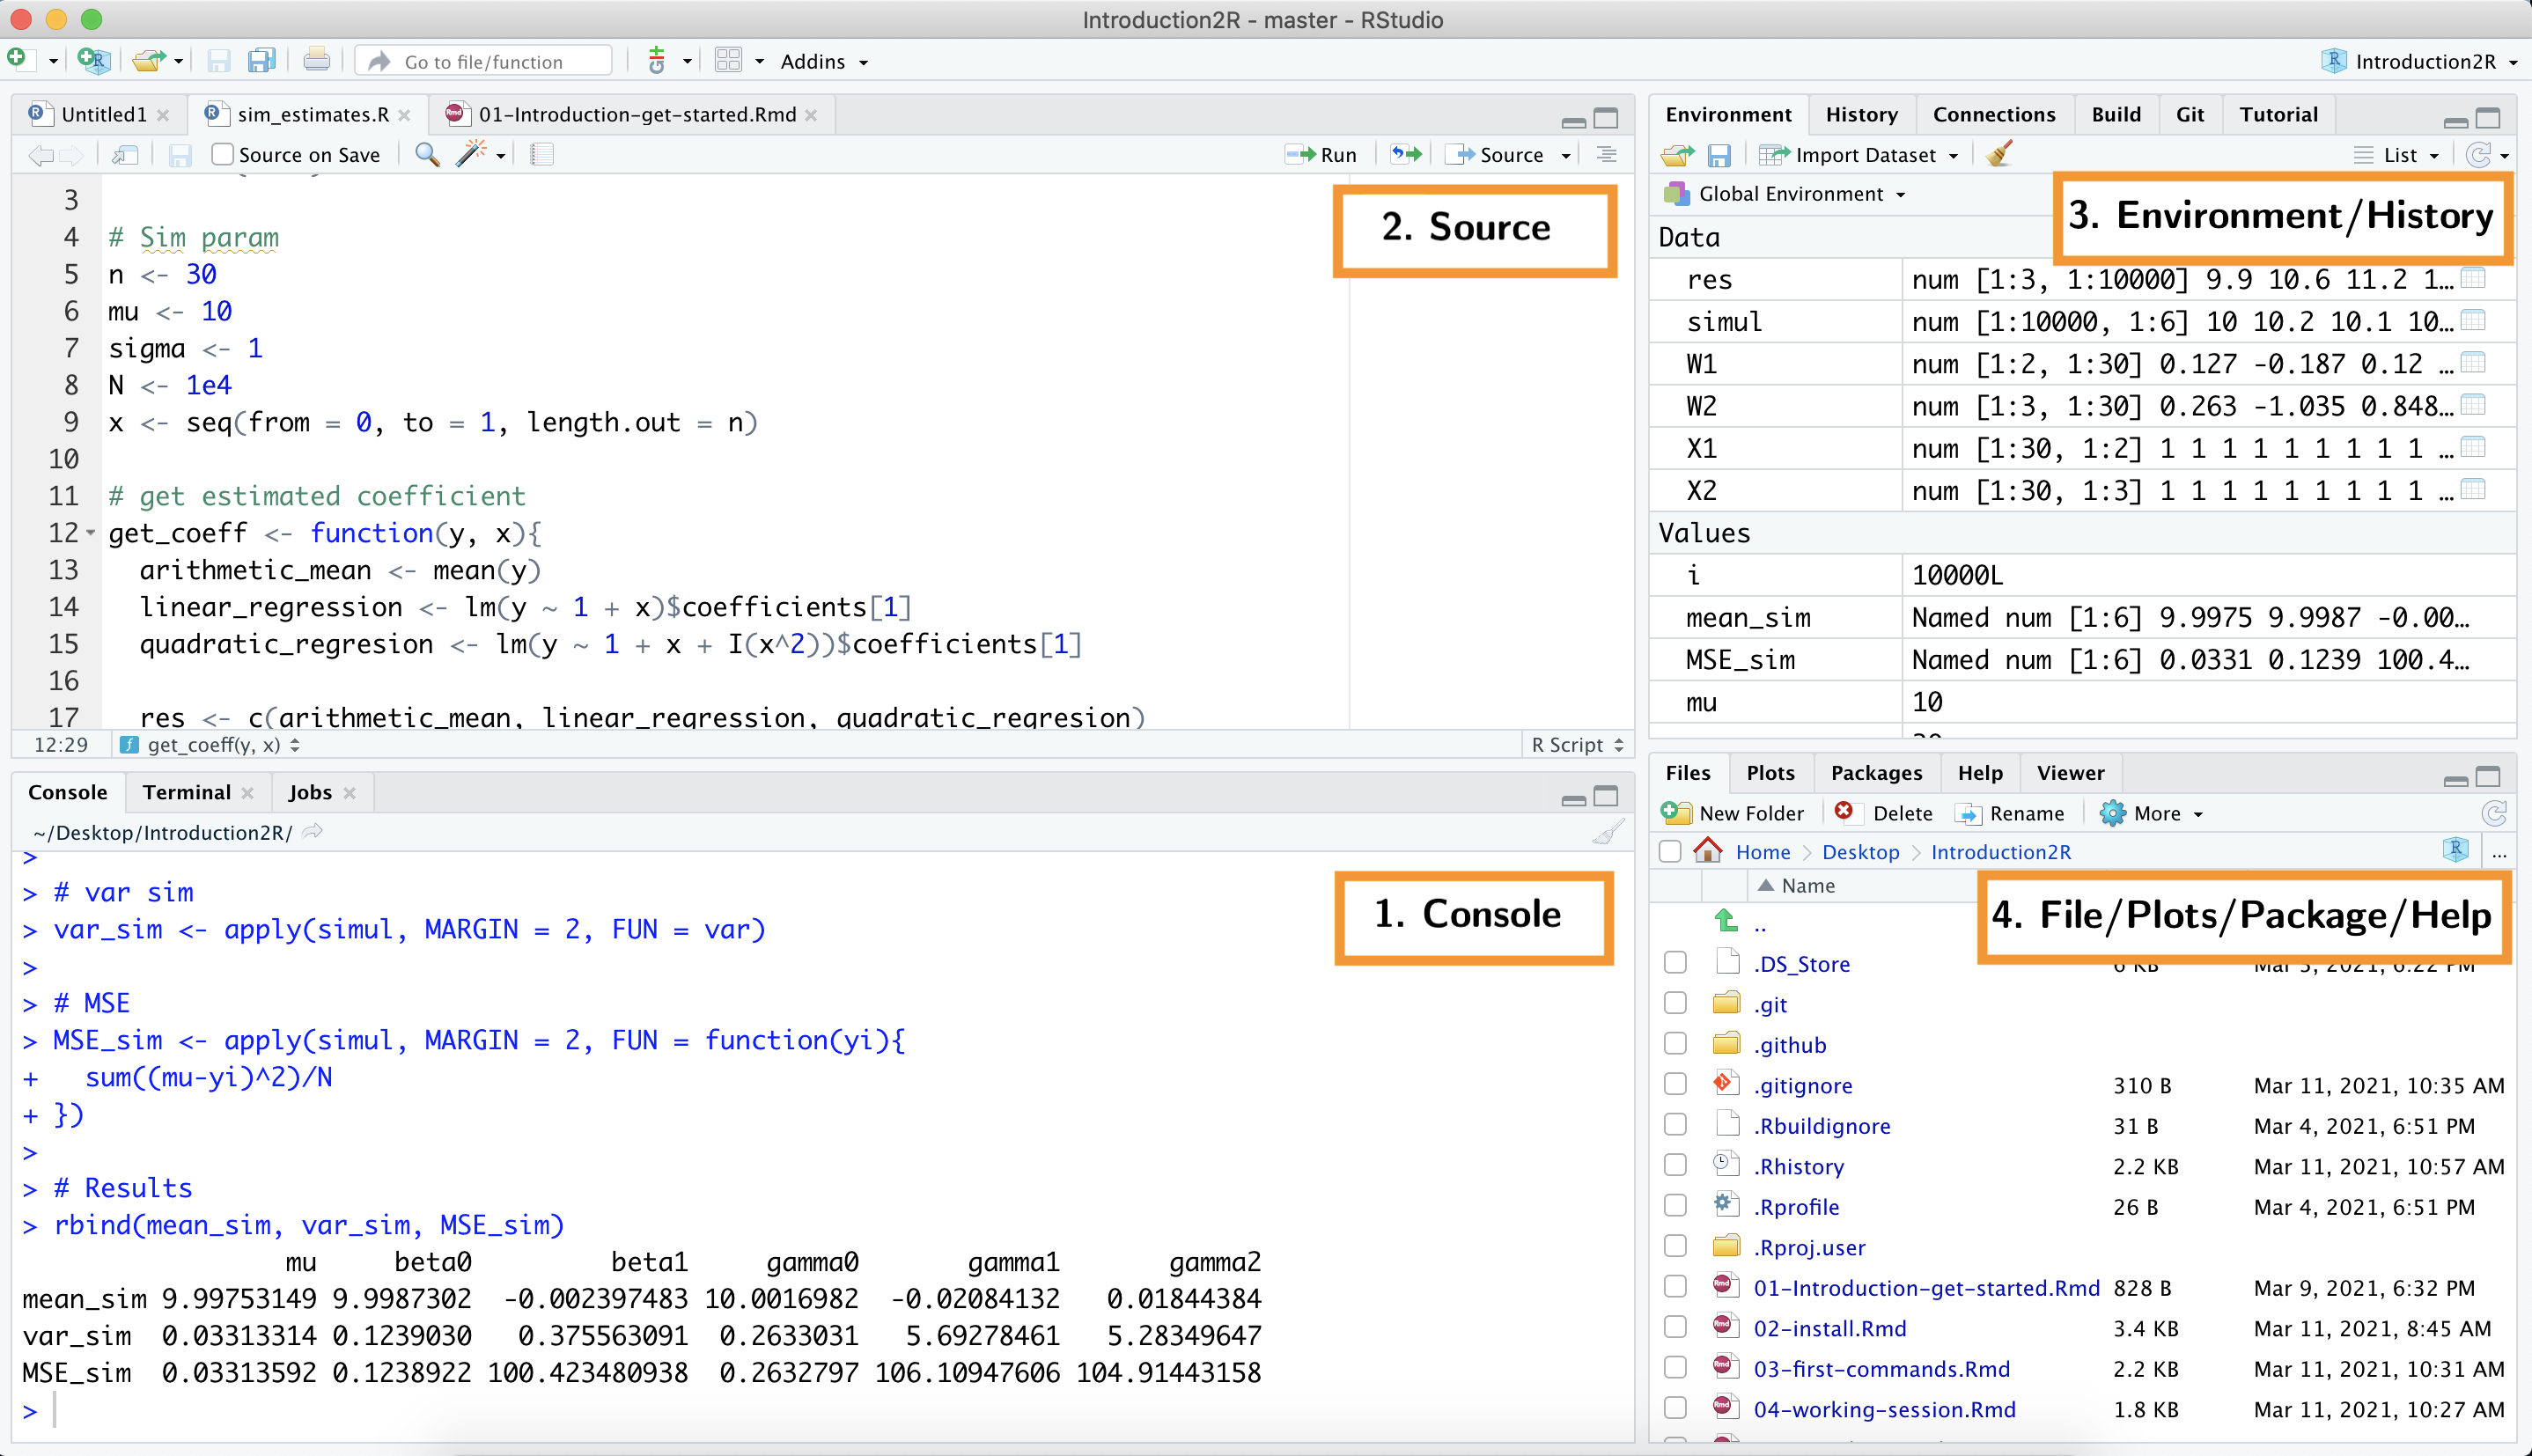
\includegraphics[width=0.85\linewidth]{images/rstudio-gui} 

}

\caption{Interfaccia utente di Rstudio con i suoi 4 pannelli}\label{fig:rstudio-gui}
\end{figure}

\hypertarget{console-il-cuore-di-r}{%
\subsubsection*{1. Console: il cuore di R}\label{console-il-cuore-di-r}}
\addcontentsline{toc}{subsubsection}{1. Console: il cuore di R}

Qui ritroviamo la \emph{Console} di R dove vengono effetivemente eseguiti tutti i tuoi codici e comandi. Nota come nell'ulitma riga della \emph{Console} appaia il carattere \texttt{\textgreater{}}. Questo è definito \emph{prompt} è ci indica che R in attesa di nuovi comandi da eseguire.

La \emph{Console} di R è un'interfaccia a linea di comando. A differenza di altri programmi ``\emph{punta e clicca}'', in R è necessario digitare i comandi utilizzando la tastiera. Per eseguire dei comandi possiamo direttamnte scrivere nella \emph{Console} le operazioni da eseguire e premere \texttt{invio}. R eseguirà immediatamente i nostro comando, riporterà il risultato e nella linea successiva apparirà nuovamente il \emph{prompt} indicando che R è pronto ad eseguire un altro comando (vedi Figura \ref{fig:comand-sequence}).

\begin{figure}

{\centering 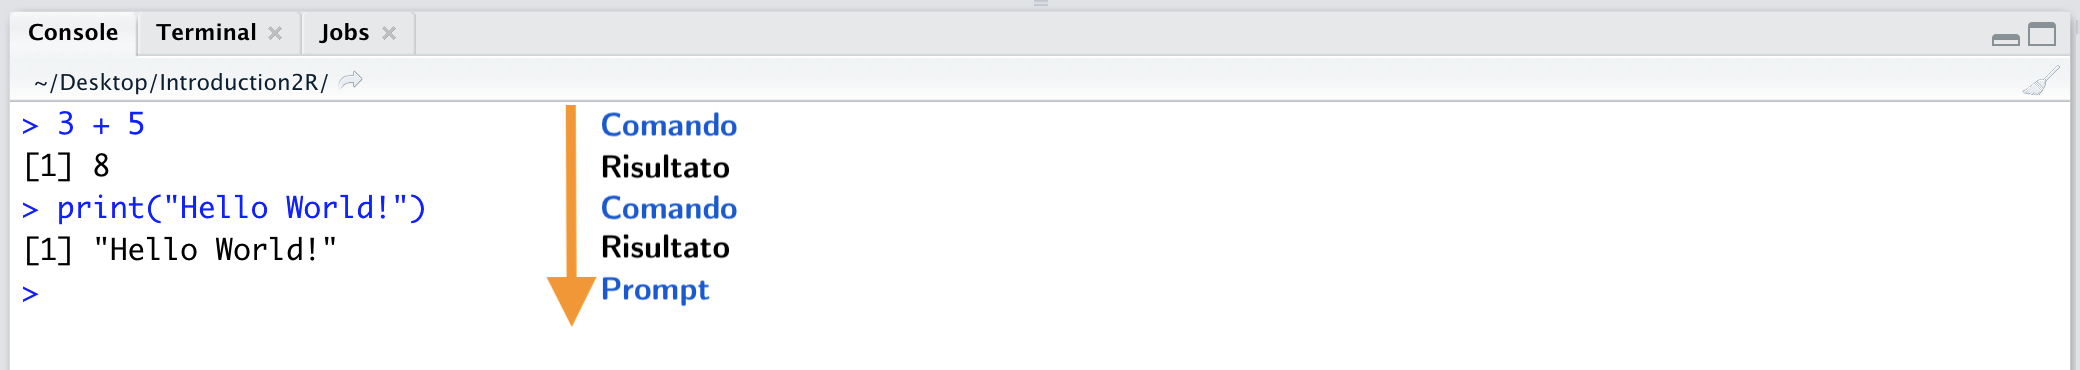
\includegraphics[width=0.95\linewidth]{images/comand-sequence} 

}

\caption{Esecuzione di comandi direttamente nella console}\label{fig:comand-sequence}
\end{figure}

Nel caso di comandi scritti su più righe, vedi l'esempio di Figura \ref{fig:multiple-line-comand}, è possibile notare come venga mostrato il simbolo \texttt{+} come \emph{prompt}. Questo indica che R è in attesa che l'intero comando venga digitato prima che esso venga eseguito.

\begin{figure}

{\centering 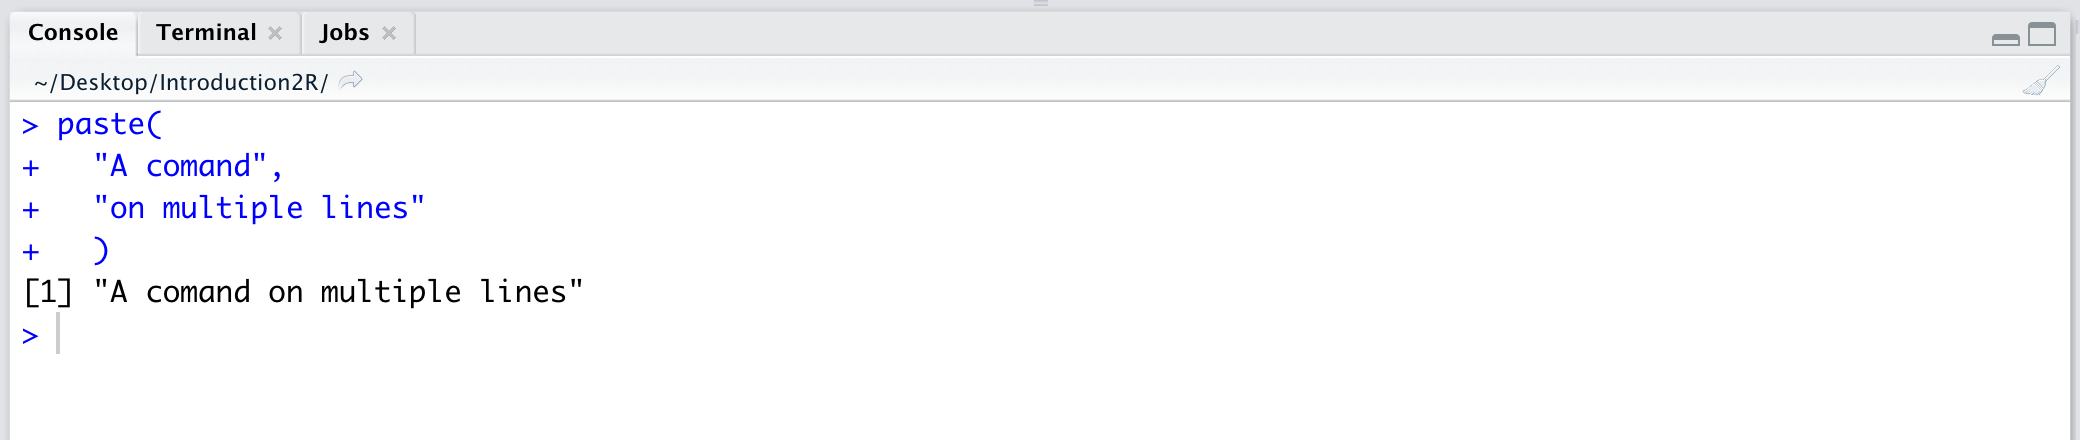
\includegraphics[width=0.95\linewidth]{images/multiple-line-comand} 

}

\caption{Esecuzione di un comando su più righe}\label{fig:multiple-line-comand}
\end{figure}

Come avrai notato facendo alcune prove, i comandi digitati nella \emph{Console} vengono eseguiti immediatamente ma non sono salvati. Per rieseguire un comando, possiamo navigare tra quelli precedentementemente eseguiti usando le freccie della tastiera \(\uparrow\downarrow\). Tuttavia, in caso di errori dovremmo riscrivere e rieseguire tutti i comandi. Siccome scrivere codici è un continuo ``\emph{try and error}'', lavorare unicamente dalla \emph{Console} diventa presto caotico. Abbiamo bisogno quindi di una soluzione che ci permetta di lavrorare più comodamente sui nostri codici e di poter salvare i nostri comandi da eseguire all'occorrenza con il giusto ordine. La soluzione sono gli \emph{Scripts} che introdurremo vedremo nella prossima sezione.

\begin{tip}[Interrompere un comando]

Potrebbe accadere che per qualche errore nel digitare un comando o perchè sono richiesti lunghi tempi computazionali, la \emph{Console} di R diventi non responsiva. In questo caso è necessario interrompere la scrittura o l'esecuzione di un comando. Vediamo due situazioni comuni:

\begin{enumerate}
\def\labelenumi{\arabic{enumi}.}
\tightlist
\item
  \textbf{Continua a comparire il prompt} \texttt{+}. Specialmente nel caso di utilizzo di parentesi e lunghi comandi, accade che una volta premuto \texttt{invio} R non esegua alcun comando ma resta in attesa mostrando il \emph{prompt} \texttt{+} (vedi Figure seguente). Questo è in genere dato da un errore nella sintassi del comando (e.g., un errore nell'uso delle parentesi o delle virgole). Per riprendere la sessione è necessario premere il tasto \texttt{esc} della tastiera. L'apprire del \emph{prompt} \texttt{\textgreater{}}, indica che R è nuovamente in ascolto pronto per esequire un nuovo comando ma attento a non ripetere lo stesso errore, la sintassi dei comandi è importante (vedi Capitolo TODO).
\end{enumerate}

\begin{center}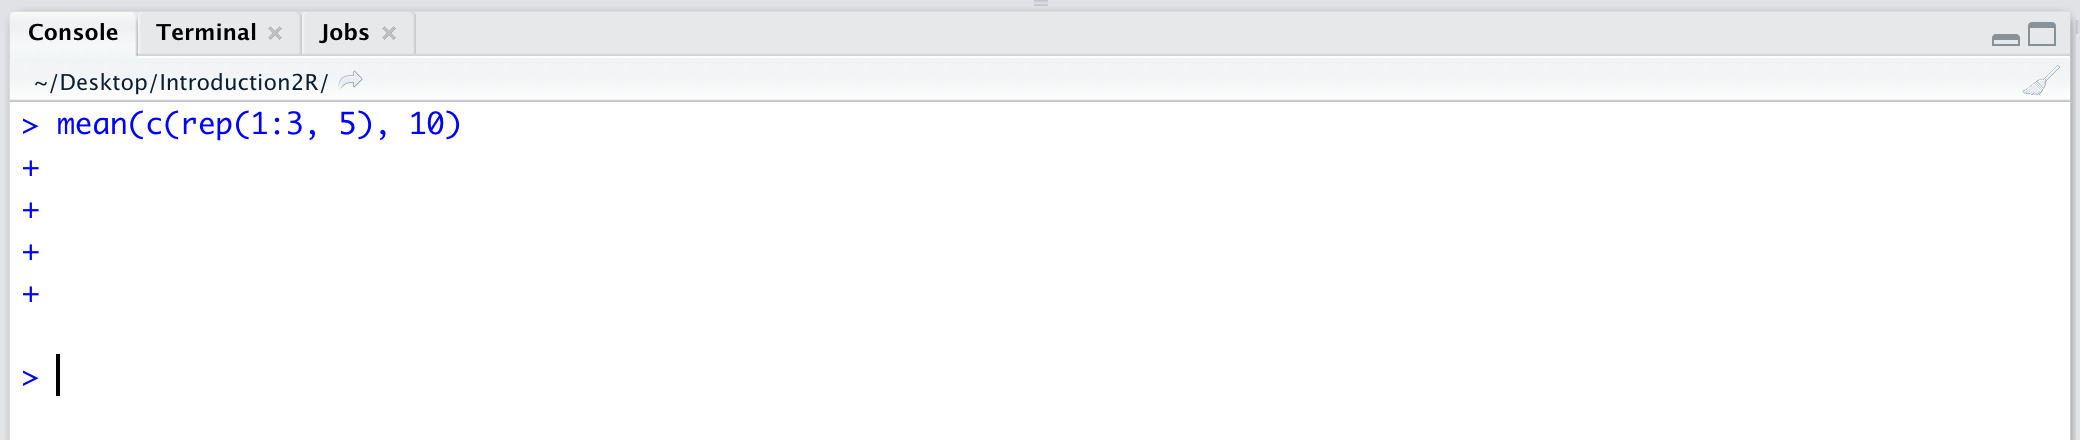
\includegraphics[width=0.95\linewidth]{images/comand-esc} \end{center}

\begin{enumerate}
\def\labelenumi{\arabic{enumi}.}
\setcounter{enumi}{1}
\tightlist
\item
  \textbf{R non risponde}. Alcuni calcoli potrebbero richiedere molto tempo o semplicemnte un qualche problema ha mandato in loop la tua sessione di lavoro. In questa situazione la \emph{Console} di R diventa non responsiva. Nel caso fosse necessario interrompere i processi attualmente in esecuzione devi premere il pulsante \emph{STOP} come indicato nella Figura seguente. R si fermerà e ritornerà in attesa di nuovi comandi (\emph{prompt} \texttt{\textgreater{}}).
\end{enumerate}

\begin{center}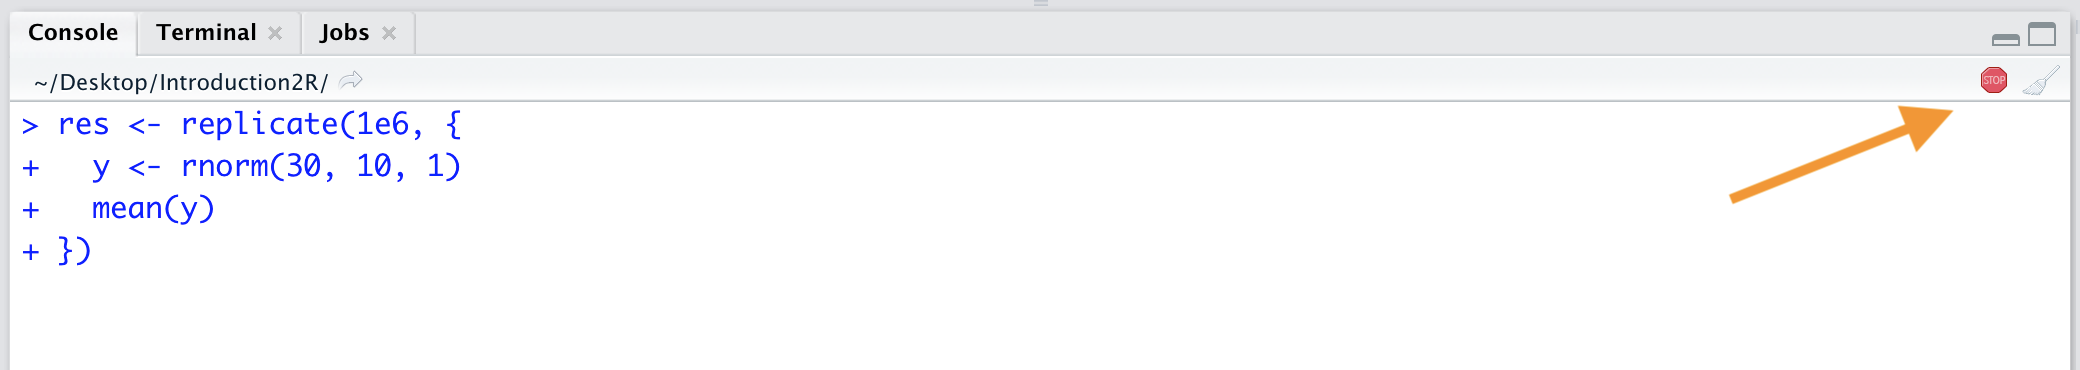
\includegraphics[width=0.95\linewidth]{images/console-stop} \end{center}

\end{tip}

\begin{trick}[Force Quit]

In alcuni casi estremi in cui R sembra non rispondere, usa i comandi \texttt{Ctrl-C} per forzare R a interrompere il processo in esecuzione.

Come ultima soluzione ricorda uno dei principi base dell'informatica ``\emph{spegni e riaccendi}'' (a volte potrebbe bastare chiudere e riaprire RStudio).

\end{trick}

\hypertarget{source-il-tuo-blocco-appunti}{%
\subsubsection*{2. Source: il tuo blocco appunti}\label{source-il-tuo-blocco-appunti}}
\addcontentsline{toc}{subsubsection}{2. Source: il tuo blocco appunti}

In questa parte vengono mostrati i tuoi \emph{Scripts}. Questi non sono altro che degli speciali documenti (con estensione ``\textbf{.R}'') in cui sono salvati i tuoi codici e comandi che potrai eseguire quando necessario in R. Gli \emph{Scripts} ti permetteranno di lavorare comodamente sui tuoi codici, scrivere i comandi, corregerli, organizzarli, aggiungere dei commenti e soprattutto salvarli.

Dopo aver terminato di scrivere i comandi, posiziona il cursore sulla stessa linea del comando che desideri eseguire e premi \texttt{command\ +\ invio} (MacOs) o \texttt{Ctrl+R} (Windows). Automaticamente il comando verà copiato nella \emph{Console} ed eseguito. In alternativa potrai premere il tasto \textbf{Run} indicato dalla freccia in Figura \ref{fig:script-run}.

\begin{figure}

{\centering 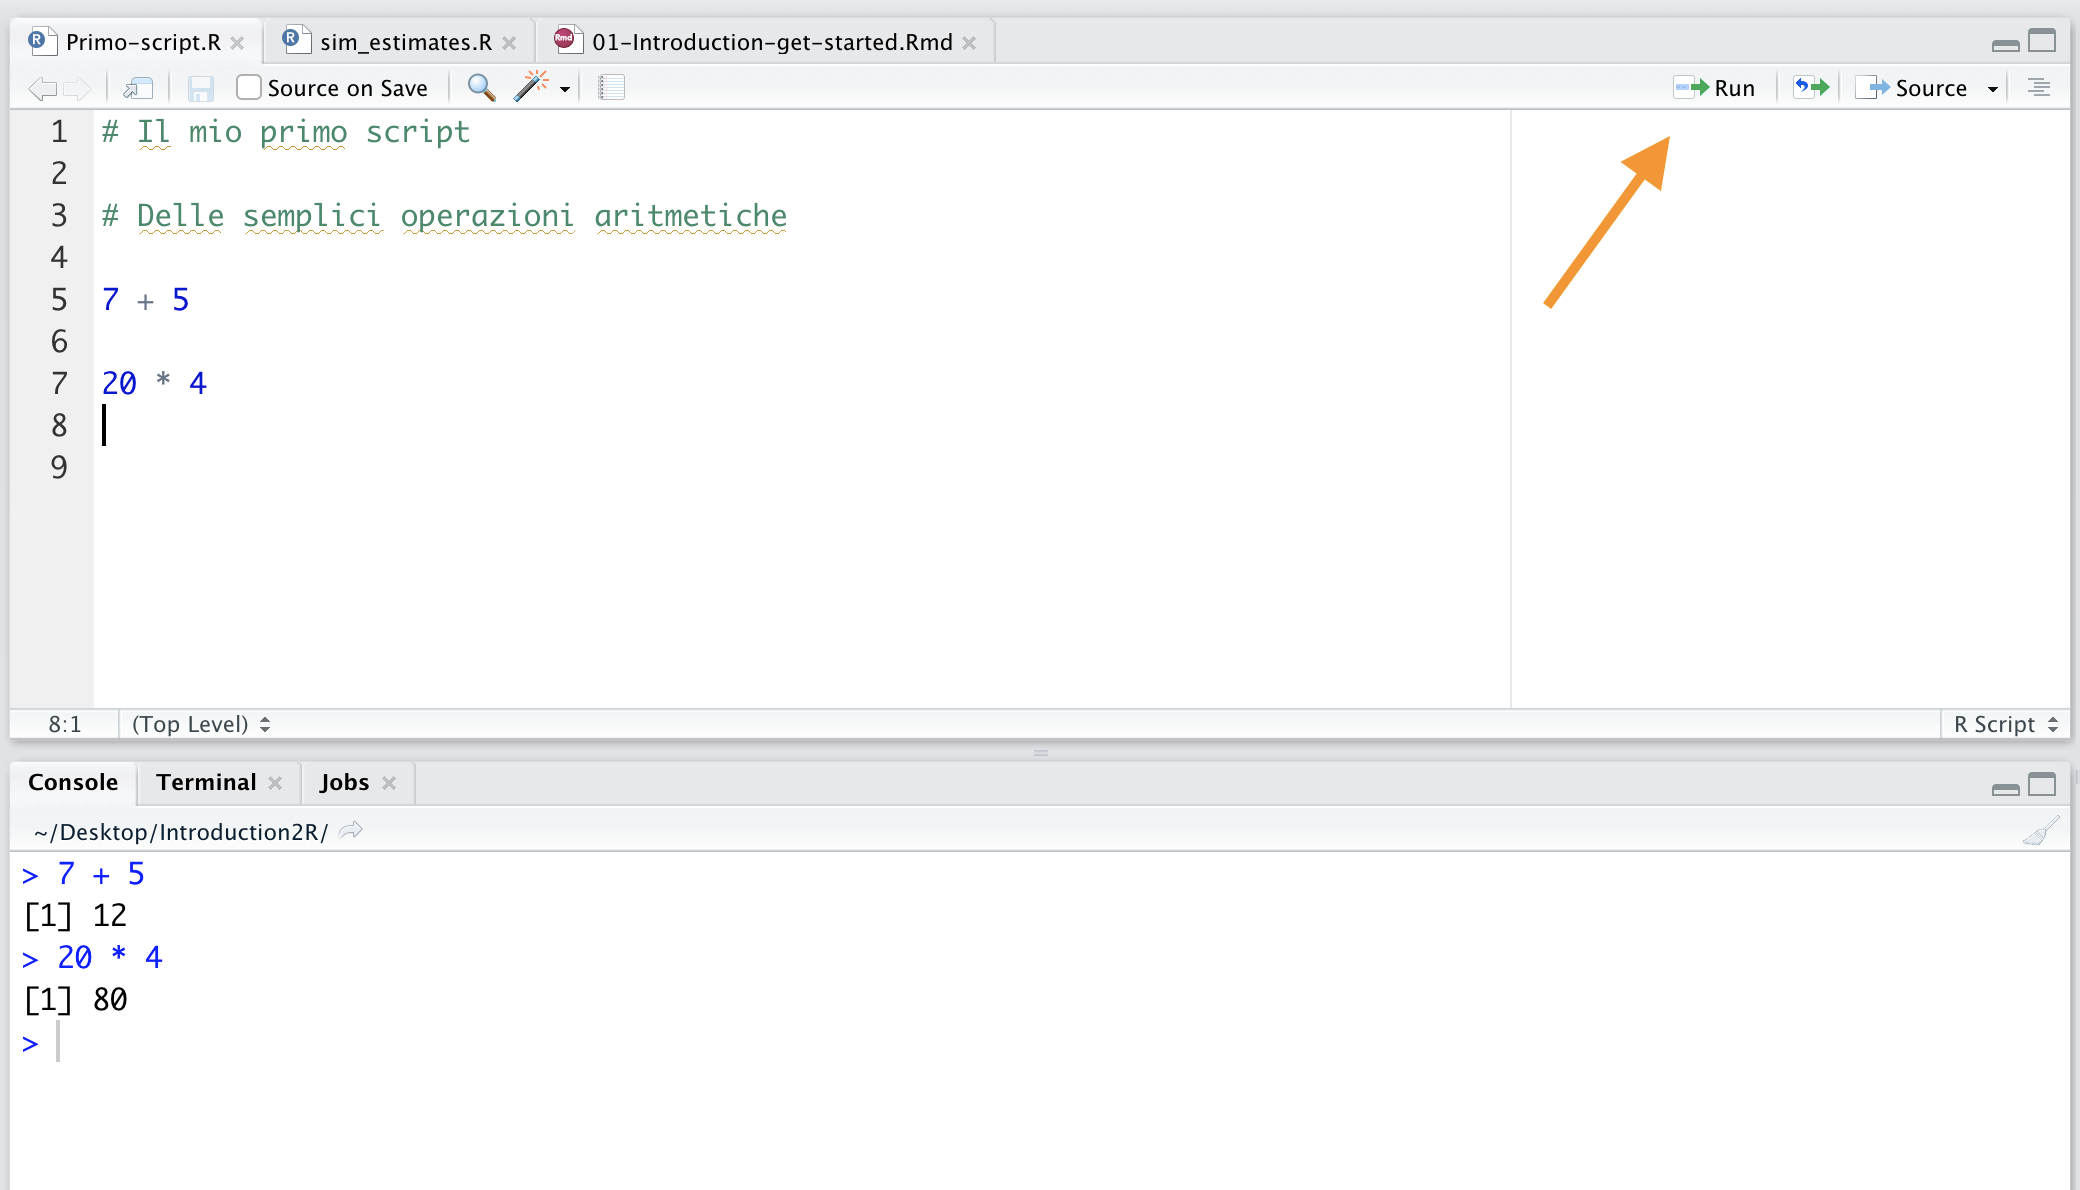
\includegraphics[width=0.95\linewidth]{images/script-run} 

}

\caption{Esecuzione di un comando da script premi `command + invio` (MacOs)/ `Ctrl+R` (Windows) o premi il tasto indicato dalla freccia}\label{fig:script-run}
\end{figure}

\begin{tip}[Commenti]

Se hai guardato con attenzione lo script rappresentato in Figura \ref{fig:script-run}, potresti aver notato delle righe di testo verde precedute dal simbolo \texttt{\#}. Questo simbolo può essere utlizzato per inserire dei \emph{commenti} all'interno dello script. R ignorerà qualsiasi commento ed eseguirà soltato le parti di codici.

L'utilizzo dei commenti è molto importante nel caso di script complessi poichè ci permette di spiegare e documentare il codice che viene eseguito. Nel Capitolo TODO approfondiremo il loro utilizzo.

\end{tip}

\hypertarget{environment-e-history-la-sessione-di-lavoro}{%
\subsubsection*{3. Environment e History: la sessione di lavoro}\label{environment-e-history-la-sessione-di-lavoro}}
\addcontentsline{toc}{subsubsection}{3. Environment e History: la sessione di lavoro}

Qui sono presentati una serie di pannelli utili per valutare informazioni inerenti alla propria sessione di lavoro. I pannelli principali sono \emph{Environment} e \emph{History} (gli altri pannelli presenti in Figura \ref{fig:environment} riguardanno funzioni avanzate di RStudio).

\begin{itemize}
\tightlist
\item
  \textbf{Environment}: elenco tutti gli oggetti e variabili attualmente presenti nel'ambiente di lavoro. Approfondiremo i concetti di variabili e di ambiente di lavoro rispettivamente nel Capitolo TODO e Capitolo TODO.
\end{itemize}

\begin{figure}

{\centering 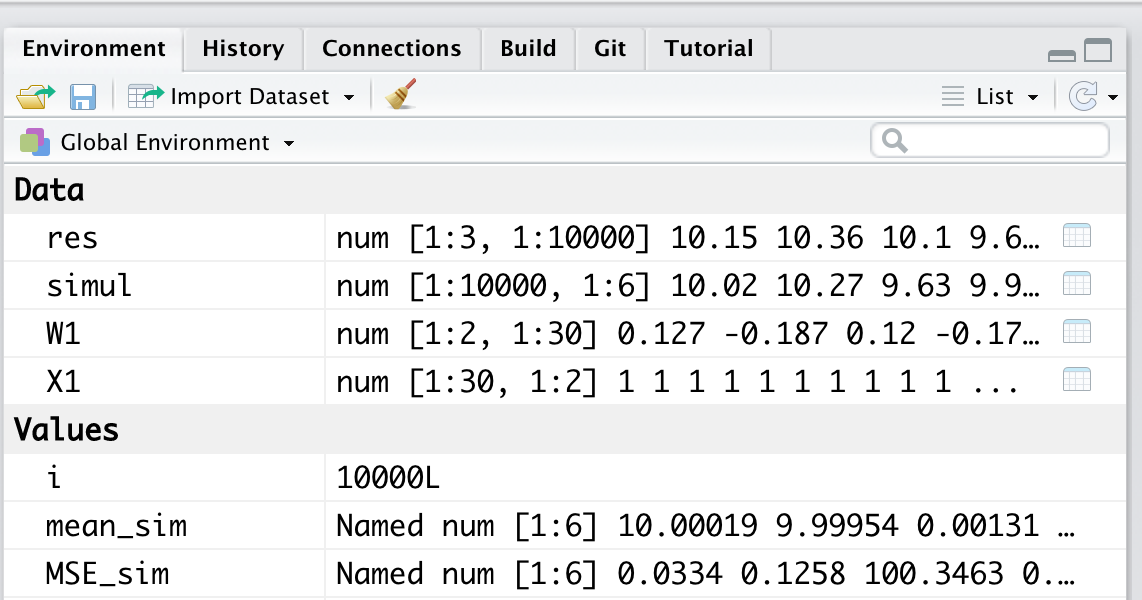
\includegraphics[width=0.6\linewidth]{images/environment} 

}

\caption{*Environment* - Elenco degli oggetti e variabili presenti nel'ambiente di lavoro}\label{fig:environment}
\end{figure}

\begin{itemize}
\tightlist
\item
  \textbf{History}: elenco di tutti i comandi precedentemente eseguiti nella console. Nota che questo no equivale ad uno script, anzi, è semplicemente un elenco non modificabile (e quasi mai usato).
\end{itemize}

\hypertarget{file-plots-package-help-system-management}{%
\subsubsection*{4. File, Plots, Package, Help: system management}\label{file-plots-package-help-system-management}}
\addcontentsline{toc}{subsubsection}{4. File, Plots, Package, Help: system management}

In questa parte sono raccolti una serie di pannelli utilizzatti per interfacciarsi con ulteriori risorse del sistema (e.g., file e pacchetti) o produrre output quali grafici e tabelle.

\begin{itemize}
\tightlist
\item
  \textbf{Files}: pannello da cui è possibile navigare tra tutti i file del proprio computer
\end{itemize}

\begin{figure}

{\centering 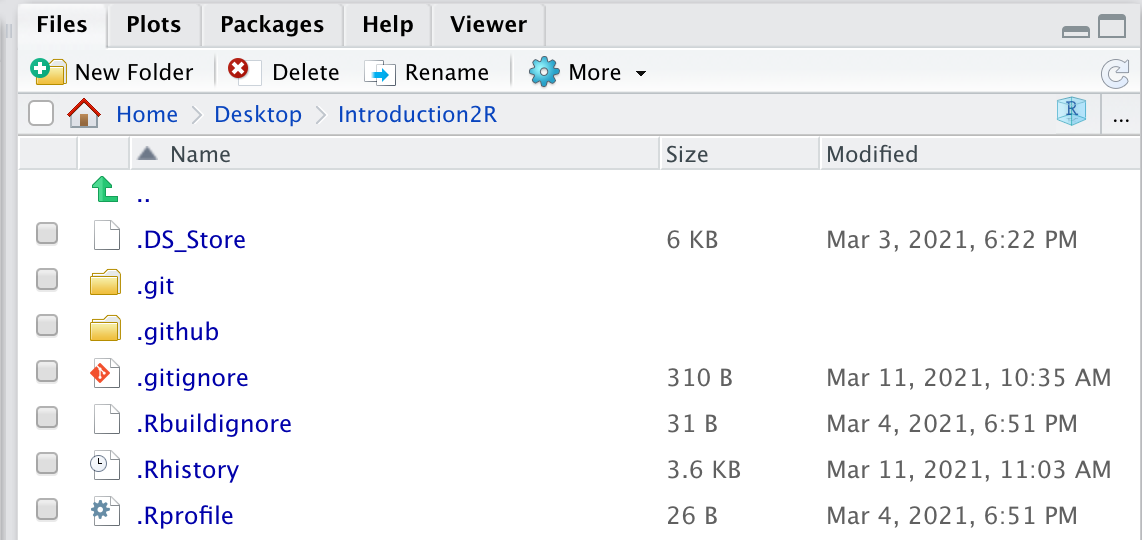
\includegraphics[width=0.6\linewidth]{images/files} 

}

\caption{*Files* - permette di navigare tra i file del proprio computer}\label{fig:files}
\end{figure}

\begin{itemize}
\tightlist
\item
  \textbf{Plots}: pannello i cui vengono prodotti i grafici e che è possibil esportare cliccando \emph{Export}.
\end{itemize}

\begin{figure}

{\centering 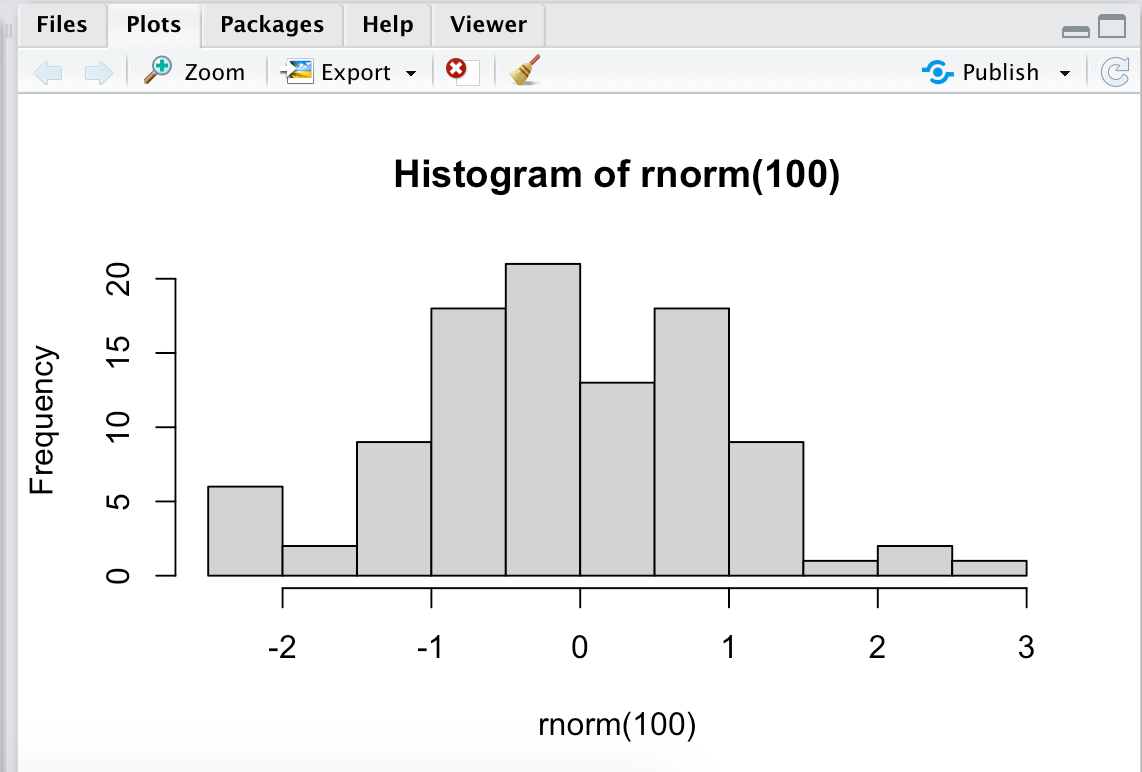
\includegraphics[width=0.6\linewidth]{images/plots} 

}

\caption{*Plots* - presentazione dei grafici}\label{fig:plots}
\end{figure}

\begin{itemize}
\tightlist
\item
  \textbf{Packages}: elenco dei pacchetti di R (questo argomento verrà approfondito nel Capitolo TODO).
\end{itemize}

\begin{figure}

{\centering 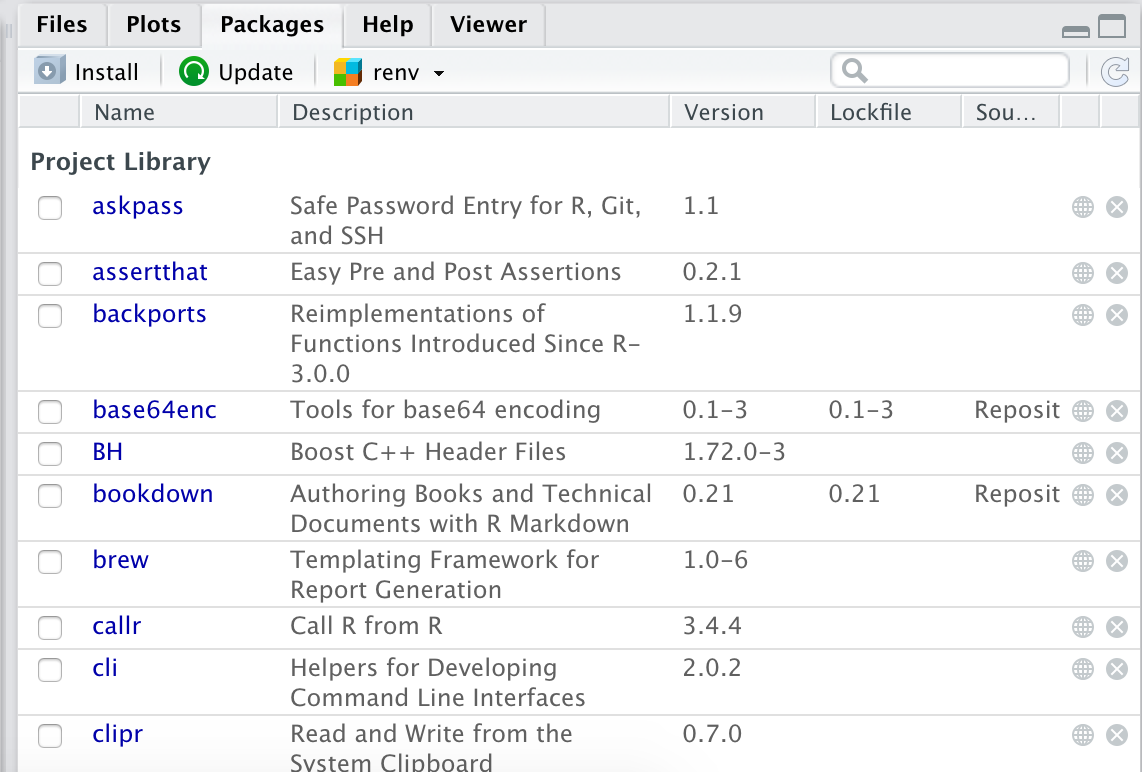
\includegraphics[width=0.6\linewidth]{images/packages} 

}

\caption{*Packages* - elenco dei pacchetti di R}\label{fig:packages}
\end{figure}

\begin{itemize}
\tightlist
\item
  \textbf{Help}: utilizzato per navigare la documentazione interna di R (questo argomento verrà approfondito nel Capitolo TODO).
\end{itemize}

\begin{figure}

{\centering 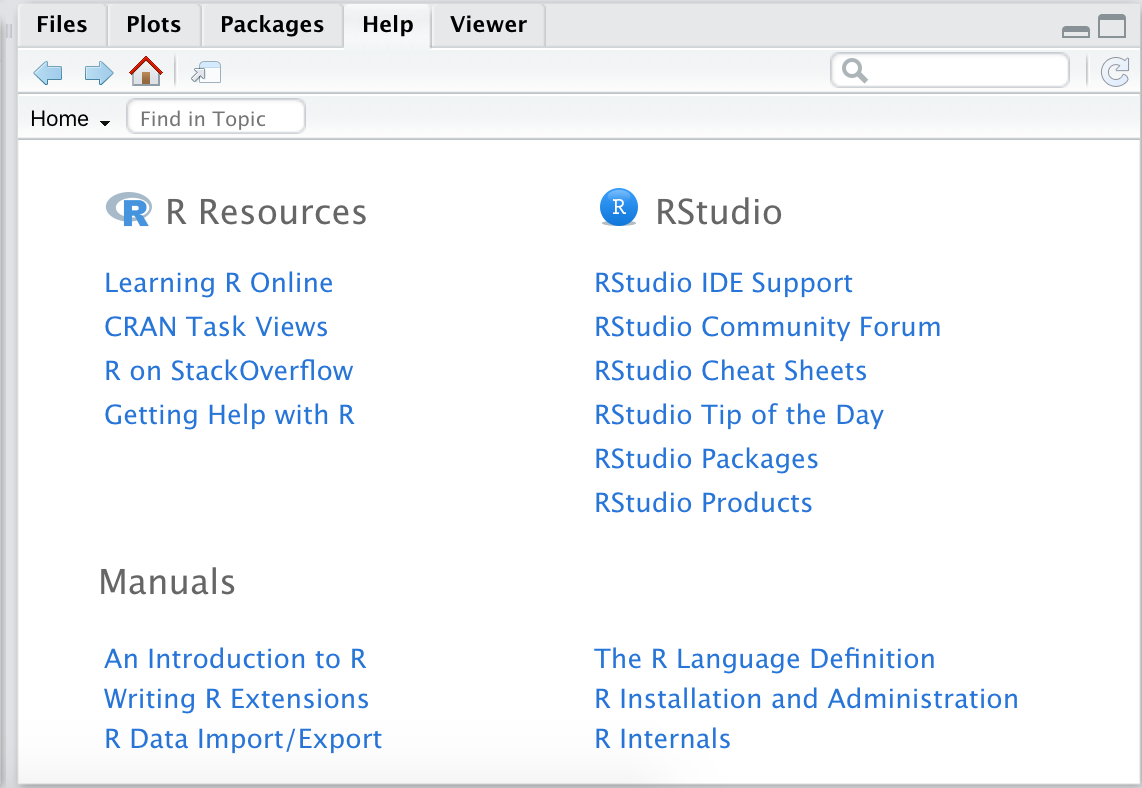
\includegraphics[width=0.6\linewidth]{images/help} 

}

\caption{*Help* -  documentazione di R}\label{fig:help}
\end{figure}

\begin{tip}[Personalizza tema e layout]

RStudio permette un ampio grado di personalizzazione dell'intrafaccia grafica utilizzata. E' possibile cambiare tema, font e disposizione dei pannelli a seconda dei tuoi gusti ed esigenze.

Prova a cambiare il tema dell editor in \emph{Idle Fingers} per utlizzare on background scuro che affatichi meno la vista (vedi Figura seguente). Clicca su RStudio \textgreater{} Preferenze \textgreater{} Appearence (MacOS) o Tools \textgreater{} Options \textgreater{} Appearence (Windows).

\begin{center}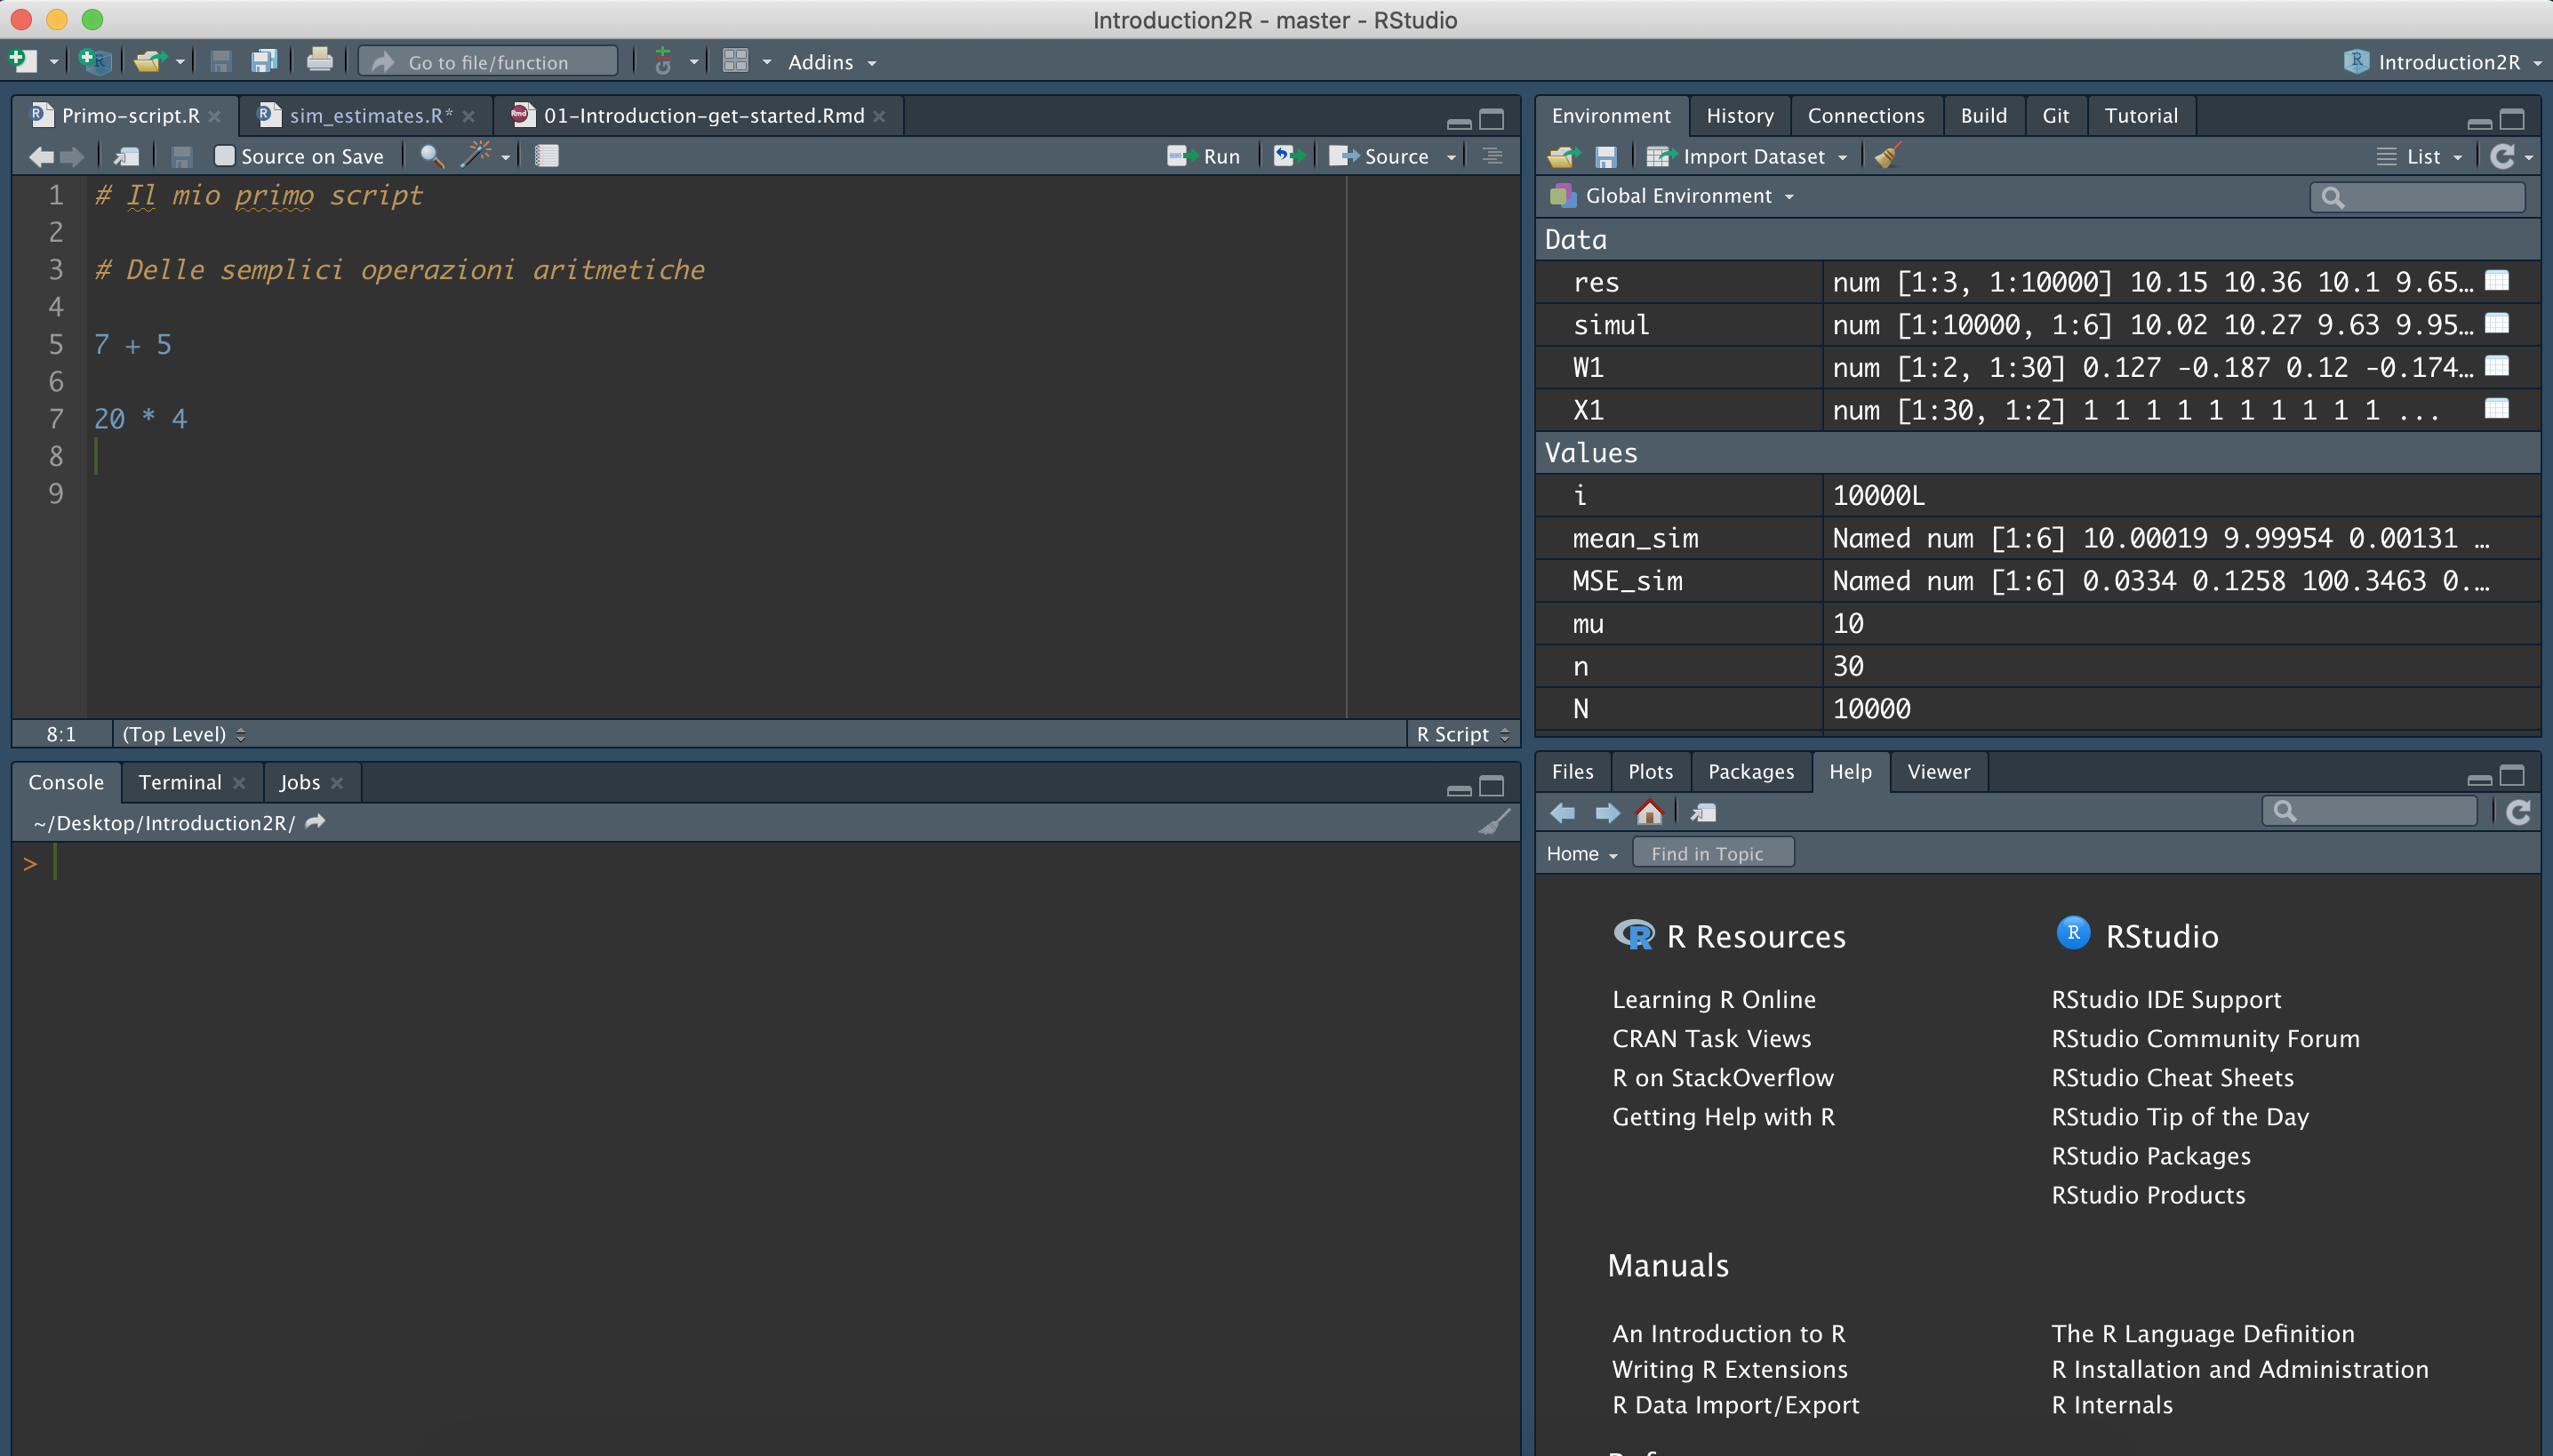
\includegraphics[width=0.9\linewidth]{images/dark-theme} \end{center}

\end{tip}

\hypertarget{first-comands}{%
\chapter{Primi Passi in R}\label{first-comands}}

In questo capitolo muoveremo i primi passi in R. Inizialmente vedremo come eseguire operazioni matematiche e logiche in R. Introdurremo successivamente l'uso delle variabili e delle funzioni in R.

Imparare R è un lungo percorso (scoop: questo percorso non termina mai dato che R è sempre in continua evoluzione). Soprattutto all'inizio può sembrare eccessivamente difficile poichè è si incontrano per la prima volta molti comandi e concetti di programmazione. Tuttavia, una volta famigliarizzato con gli apetti di base, la progressione diventa sempre più veloce (inarrestabile direi!).

In questo capitolo introdurremo per la prima volta molti elementi che saranno poi ripresi e approfonditi nei seguenti capitoli. Quindi non preoccuparti se non tutto ti sarà chiaro fin da subito. Imparare il tuo primo linguaggio di programmazione è difficile ma da qualche parte bisogna pure iniziare. Pronto per le tue prime linee di codice? Let's become a useR!

Ora che abbiamo iniziato a famigliarizzare con il nostro stumento di lavoro possimao finalmente dare fuoco alle polveri e concentraci sulla scrittura di codici!

\hypertarget{operatori-matematici}{%
\section{Operatori Matematici}\label{operatori-matematici}}

\hypertarget{operatori-logici}{%
\section{Operatori Logici}\label{operatori-logici}}

\hypertarget{approfondimento-operatore-in}{%
\subsubsection{\texorpdfstring{approfondimento operatore \texttt{\%in\%}}{approfondimento operatore \%in\%}}\label{approfondimento-operatore-in}}

\hypertarget{creazione-di-variabili}{%
\section{Creazione di Variabili}\label{creazione-di-variabili}}

concetto di variabile e assegnare i valori

\hypertarget{approfondimento-diversi-modi-di-assegnare-un-valore---assign}{%
\subsubsection{\texorpdfstring{approfondimento diversi modi di ``assegnare un valore'' (\texttt{\textless{}-}, \texttt{=}, \texttt{assign()})}{approfondimento diversi modi di ``assegnare un valore'' (\textless-, =, assign())}}\label{approfondimento-diversi-modi-di-assegnare-un-valore---assign}}

\hypertarget{utilizzo-di-funzioni}{%
\section{Utilizzo di funzioni}\label{utilizzo-di-funzioni}}

\hypertarget{section}{%
\subsection{}\label{section}}

\hypertarget{part-struttura-dati}{%
\part*{Struttura Dati}\label{part-struttura-dati}}
\addcontentsline{toc}{part}{Struttura Dati}

\hypertarget{introduzione}{%
\chapter*{Introduzione}\label{introduzione}}
\addcontentsline{toc}{chapter}{Introduzione}

Working in progress.

\hypertarget{working-session}{%
\chapter{Sessione di Lavoro}\label{working-session}}

Working in progress.

\hypertarget{infobox}{%
\section{Infobox}\label{infobox}}

Illustrations included in \texttt{images/} are retrieved from \href{https://rstudio4edu.github.io/rstudio4edu-book/}{rstudio4edu-book} under \href{https://creativecommons.org/licenses/by-nc/2.0/}{CC-BY-NC}. Remember to include an \emph{Attributions} section in the book and repository's README file.

\begin{tip}[My title]

Lorem ipsum dolor sit amet consectetur adipisicing elit. Maxime mollitia,
molestiae quas vel sint commodi repudiandae consequuntur voluptatum laborum
numquam blanditiis harum quisquam eius sed odit fugiat iusto fuga praesentium
optio, eaque rerum!

\end{tip}

\begin{warning}[My title]

Lorem ipsum dolor sit amet consectetur adipisicing elit. Maxime mollitia,
molestiae quas vel sint commodi repudiandae consequuntur voluptatum laborum
numquam blanditiis harum quisquam eius sed odit fugiat iusto fuga praesentium
optio, eaque rerum!

\end{warning}

\begin{deffun}[My title]

Lorem ipsum dolor sit amet consectetur adipisicing elit. Maxime mollitia,
molestiae quas vel sint commodi repudiandae consequuntur voluptatum laborum
numquam blanditiis harum quisquam eius sed odit fugiat iusto fuga praesentium
optio, eaque rerum!

\end{deffun}

\begin{design}[My title]

Lorem ipsum dolor sit amet consectetur adipisicing elit. Maxime mollitia,
molestiae quas vel sint commodi repudiandae consequuntur voluptatum laborum
numquam blanditiis harum quisquam eius sed odit fugiat iusto fuga praesentium
optio, eaque rerum!

\end{design}

\begin{trick}[My title]

Lorem ipsum dolor sit amet consectetur adipisicing elit. Maxime mollitia,
molestiae quas vel sint commodi repudiandae consequuntur voluptatum laborum
numquam blanditiis harum quisquam eius sed odit fugiat iusto fuga praesentium
optio, eaque rerum!

\end{trick}

\hypertarget{problema-google-soluzione}{%
\section{Problema + Google = Soluzione}\label{problema-google-soluzione}}

Quando si approccia la scrittura di codice, anche molto semplice la cosa che sicuramente capiterà più spesso sarà riscontrare \textbf{errori} e quindi trovare il modo per risolverli.

\begin{quote}
Qualche programmatore esperto direbbe che l'essenza stessa di programmare è in realtà risolvere gli errori che il codice produce.
\end{quote}

L'\textbf{errore non è quindi un difetto o un imprevisto}, ma parte integrante della scrittura del codice. L'importante è capire come gestirlo.

Abbiamo tutti le immagini in testa di programmatori da film che scrivono codice alla velocità della luce, quando nella realtà dobbiamo spesso affrontare \textbf{bug}, \textbf{errori di output} o altri problemi vari. Una serie di skills utili da imparare sono:

\begin{itemize}
\tightlist
\item
  Comprendere a fondo gli \textbf{errori} (non banale)
\item
  Sapere \textbf{come e dove cercare una soluzione} (ancora meno banale)
\item
  In caso non si trovi una soluzione direttamente, chiedere aiuto in modo efficace
\end{itemize}

\hypertarget{comprendere-gli-errori}{%
\subsubsection*{Comprendere gli errori}\label{comprendere-gli-errori}}
\addcontentsline{toc}{subsubsection}{Comprendere gli errori}

Rispetto agli errori, R è solitamente abbastanza esplicito nel farci capire il problema. Ad esempio usare una funzione di un pacchetto che non è stato caricato di solito fornisce un messaggio del tipo \texttt{Error\ in\ funzione\ :\ could\ not\ find\ function\ "funzione"}.

\hypertarget{ricercare-soluzioni}{%
\subsubsection*{Ricercare soluzioni}\label{ricercare-soluzioni}}
\addcontentsline{toc}{subsubsection}{Ricercare soluzioni}

Altre situazioni o messaggi potrebbero non essere altrettanto immediati, in quel caso Google è il nostro miglior amico.

Cercando infatti il messaggio di errore/warning su Google, al 99\% avremo altre persone che hanno avuto lo stesso problema e probabilmente anche una soluzione.

\begin{trick}[Ricerca su Google]

Il modo migliore per cercare è copiare e incollare su Google direttamente l'output di errore di R come ad esempio \texttt{Error\ in\ funzione\ :\ could\ not\ find\ function\ "funzione"} piuttosto che descrivere a parole il problema. I messaggi di errore sono standard per tutti, la tua descrizione invece no.

\end{trick}

Cercando in questo modo vedrete che molti dei risultati saranno esattamente riferiti al vostro errore:

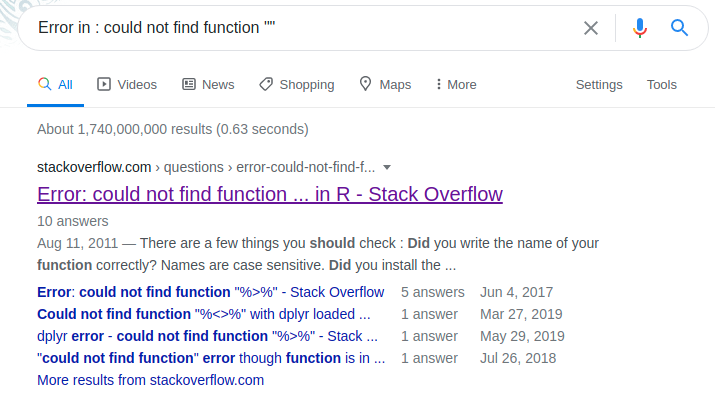
\includegraphics{images/stack_question.png}

\hypertarget{chiedere-una-soluzione}{%
\subsubsection{Chiedere una soluzione}\label{chiedere-una-soluzione}}

Se invece il vostro probelma non è un messaggio di errore ma un utilizzo specifico di R allora il consiglio è di usare una ricerca del tipo: \texttt{argomento\ +\ breve\ descrizione\ problema\ +\ R}. Nelle sezioni successive vedrete nel dettaglio altri aspetti della programmazione ma se volete ad esempio calcolare la \textbf{media} in R potrete scrivere \texttt{compute\ mean\ in\ R}.
Mi raccomando, fate tutte le ricerche in \textbf{inglese} perchè le possibilità di trovare una soluzione sono molto più alte.

Dopo qualche ricerca, vi renderete conto che il sito che vedrete più spesso si chiama \href{https://stackoverflow.com/}{\textbf{Stack Overflow}}. Questo è una manna dal cielo per tutti i programmatori, a qualsiasi livello di expertise. E' una community dove tramite domande e risposte, si impara a risolvere i vari problemi ed anche a trovare nuovi modi di fare la stessa cosa. E' veramente utile oltre che un ottimo modo per imparare.

L'ultimo punto di questa piccola guida alla ricerca di soluzioni, riguarda il fatto di dover non solo cercare ma anche chiedere. Dopo aver cercato vari post di persone che richiedevano aiuto per un problema noterete che le domande e le risposte hanno sempre una struttura simile. Questo non è solo un fatto stilistico ma anzi è molto utile per uniformare e rendere chiara la domanda ma sopratutto la risposta, in uno spirito di condivisione. C'è anche una \href{https://stackoverflow.com/help/how-to-ask}{guida dedicata} per scrivere la domanda perfetta.

In generale\footnote{Fonte: \href{https://codeblog.jonskeet.uk/2010/08/29/writing-the-perfect-question/}{Writing the perfect question - Jon Skeet}}:

\begin{itemize}
\tightlist
\item
  Titolo: un super riassunto del problema
\item
  Contesto: linguaggio (es. R), quale sistema operativo (es. Windows)
\item
  Descrizione del problema/richiesta: in modo chiaro e semplice ma non troppo generico
\item
  Codice ed eventuali dati per capire il problema
\end{itemize}

L'ultimo punto di questa lista è forse il più importante e si chiama in gergo tecnico \href{https://community.rstudio.com/t/faq-whats-a-reproducible-example-reprex-and-how-do-i-create-one/5219}{\textbf{REPREX}} (\textbf{Rep}roducible \textbf{Ex}ample). E' un tema leggermente più avanzato ma l'idea di fondo è quella di fornire tutte le informazioni possibili per poter riprodurre (e quindi eventualmente trovare una soluzione) il codice di qualcuno nel proprio computer.

Se vi dico ``R non mi fa creare un nuovo oggetto, quale è l'errore?'' è diverso da dire ``il comando \texttt{oggetto\ -\textgreater{}\ 10} mi da questo errore \texttt{Error\ in\ 10\ \textless{}-\ oggetto\ :\ invalid\ (do\_set)\ left-hand\ side\ to\ assignment}, come posso risolvere?''

\begin{tip}[My title]

Ci sono anche diversi pacchetti in R che rendono automatico creare questi esempi di codice da poter condividere, come il pacchetto \href{https://www.tidyverse.org/help/}{\texttt{reprex}}.

\end{tip}

\hypertarget{vector}{%
\chapter{Vettori}\label{vector}}

Working in progress.

\hypertarget{matrix}{%
\chapter{Matrici}\label{matrix}}

Working in progress.

\hypertarget{dataframe}{%
\chapter{Dataframe}\label{dataframe}}

Working in progress.

\hypertarget{list}{%
\chapter{Liste}\label{list}}

Working in progress.

\hypertarget{part-algoritmi}{%
\part*{Algoritmi}\label{part-algoritmi}}
\addcontentsline{toc}{part}{Algoritmi}

\hypertarget{introduzione-1}{%
\chapter*{Introduzione}\label{introduzione-1}}
\addcontentsline{toc}{chapter}{Introduzione}

Working in progress.

\hypertarget{functions}{%
\chapter{Definizione di Funzioni}\label{functions}}

Working in progress.

\hypertarget{coditionals}{%
\chapter{Programmazione Condizionale}\label{coditionals}}

Working in progress.

\hypertarget{loop}{%
\chapter{Attenti al loop}\label{loop}}

Working in progress.

\hypertarget{part-case-study}{%
\part*{Case study}\label{part-case-study}}
\addcontentsline{toc}{part}{Case study}

\hypertarget{introduzione-2}{%
\chapter*{Introduzione}\label{introduzione-2}}
\addcontentsline{toc}{chapter}{Introduzione}

Working in progress.

\hypertarget{attachment}{%
\chapter{Caso Studio I: Attaccamento}\label{attachment}}

Working in progress.

  \bibliography{book.bib,packages.bib}

\end{document}
